\documentclass[10pt,a4paper]{article}
\usepackage[utf8]{inputenc}
\usepackage[polish]{babel}
\usepackage[T1]{fontenc}
\usepackage{graphicx}
\usepackage[left=2cm,right=2cm,top=2cm,bottom=2cm]{geometry}
\usepackage{float}
\usepackage{amsmath}
\author{Adam Syrek, Poncjusz Piłat i Michał Drobniak \\ (wspomagani notatkami Sylwii i innych zacnych osób)}
\title{Opracowanie pytań na egzamin z Układów Elektronicznych}
\renewcommand\arraystretch{2}
\begin{document}
\maketitle

\newpage
\tableofcontents
\newpage
\section{Modele tranzystorów}
\subsection{Model małosygnałowy tranzystora bipolarnego}
\begin{figure}[H]
\centering
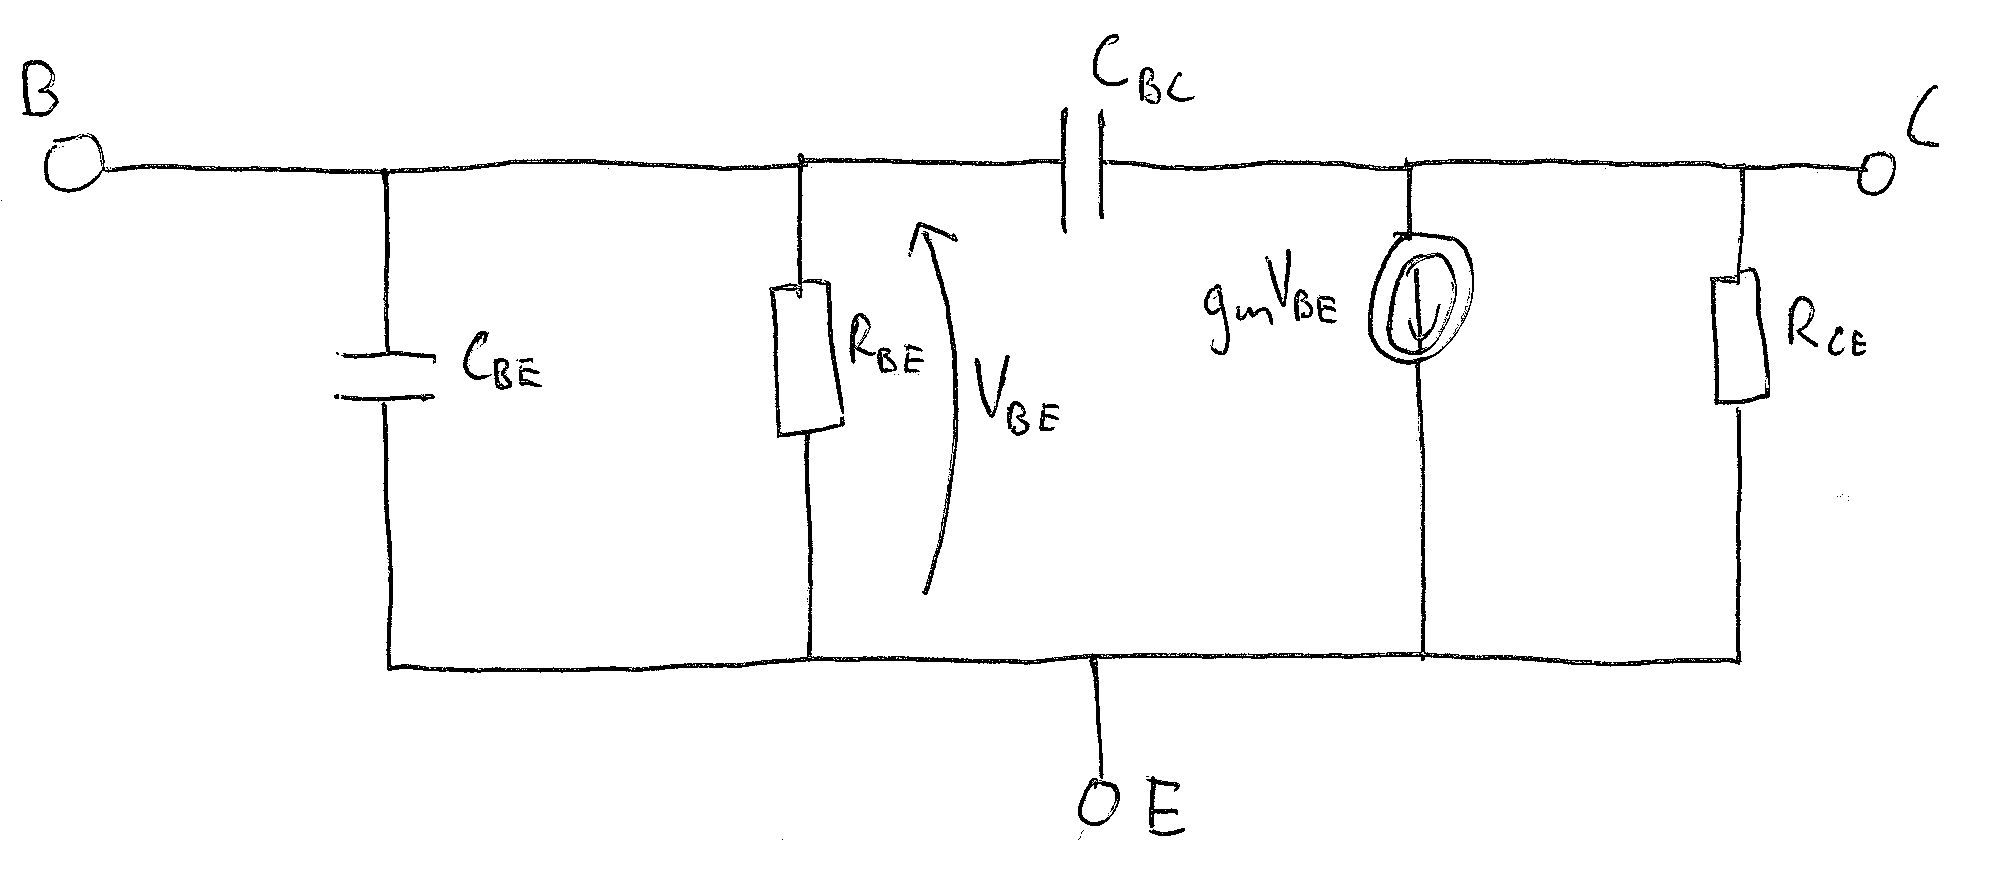
\includegraphics[width=0.7\textwidth]{malosyg_bip.png}
\end{figure}

W sumie chyba ważny wzór:
\begin{equation}
I_c = I_s(1+{V_{CE}\over V_A})e^{V_{BE} \over V_T}
\end{equation}
$V_A$ to napięcie jakiegoś Early'ego, a $V_T$ to oczywiście termiczne. Z wzoru wynika, że 
e prądu wzrasta eksponencjalnie do namięcia sterującego. Uwaga jest taka, że to jest wzór empiryczny, a nie teoretyczny, pokazuje pi razy oko zachowanie tranzystora.\\
Włąściwa polaryzacja tranzystora bipolarnego:
\begin{center}
\begin{tabular}{c|c|c}
& npn & pnp \\
\hline
$V_{BE}$ & $\geq 0.7V$ & $\leq -0.7V$ \\ 

<<<<<<< HEAD
$V_{CE}$ & $> -200mV$ & $< 200mV$\\ 
=======
$V_{CE}$ & $> 200mV$ & $< -200mV$\\ 
>>>>>>> f02f437d9ed2df267bbfc5195056d09685993dba
\end{tabular}
\end{center}

\begin{figure}[H]
\centering
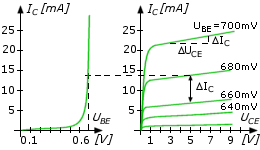
\includegraphics[width=0.5\textwidth]{char.png}
\end{figure}

Obrazek niezbyt fortunny, ale taki znalazłem. Na lewym wykresie tam gdzie prąd idzie tak ostro w górę jest obszar triodowy, potem ($V_{CE} > 200mV$) jest obszar aktywny normalny. To, że ta charakterystyka rośnie w obszarze normalnym jest spowodowane tym napięciem Early'ego we wzorze (tak zrozumiałem). W pierszym przybliżeniu to olaliśmy i w obszarze aktywnym charakterystyka była stała.\\


$g_m$ - transkonduktancja

\begin{equation}
g_m = {\partial I_C \over \partial V_{BE}} = {I_c \over V_T}
\end{equation}

Czemu tak jest, nie wiem. Wszystkie oznaczenia typu $I_C$, czy $V_{BE}$ należy odczytywać przez skróty poszczególnych części tranzystora. Wszyscy powinni to wiedzieć, ale dla zasady już dam:
\begin{itemize}
\item C - kolektor
\item B - baza
\item E - emiter (to ze strzałką na schemacie)
\end{itemize}



\subsection{Model małosygnałowy tranzystora polowego}
\begin{figure}[H]
\centering
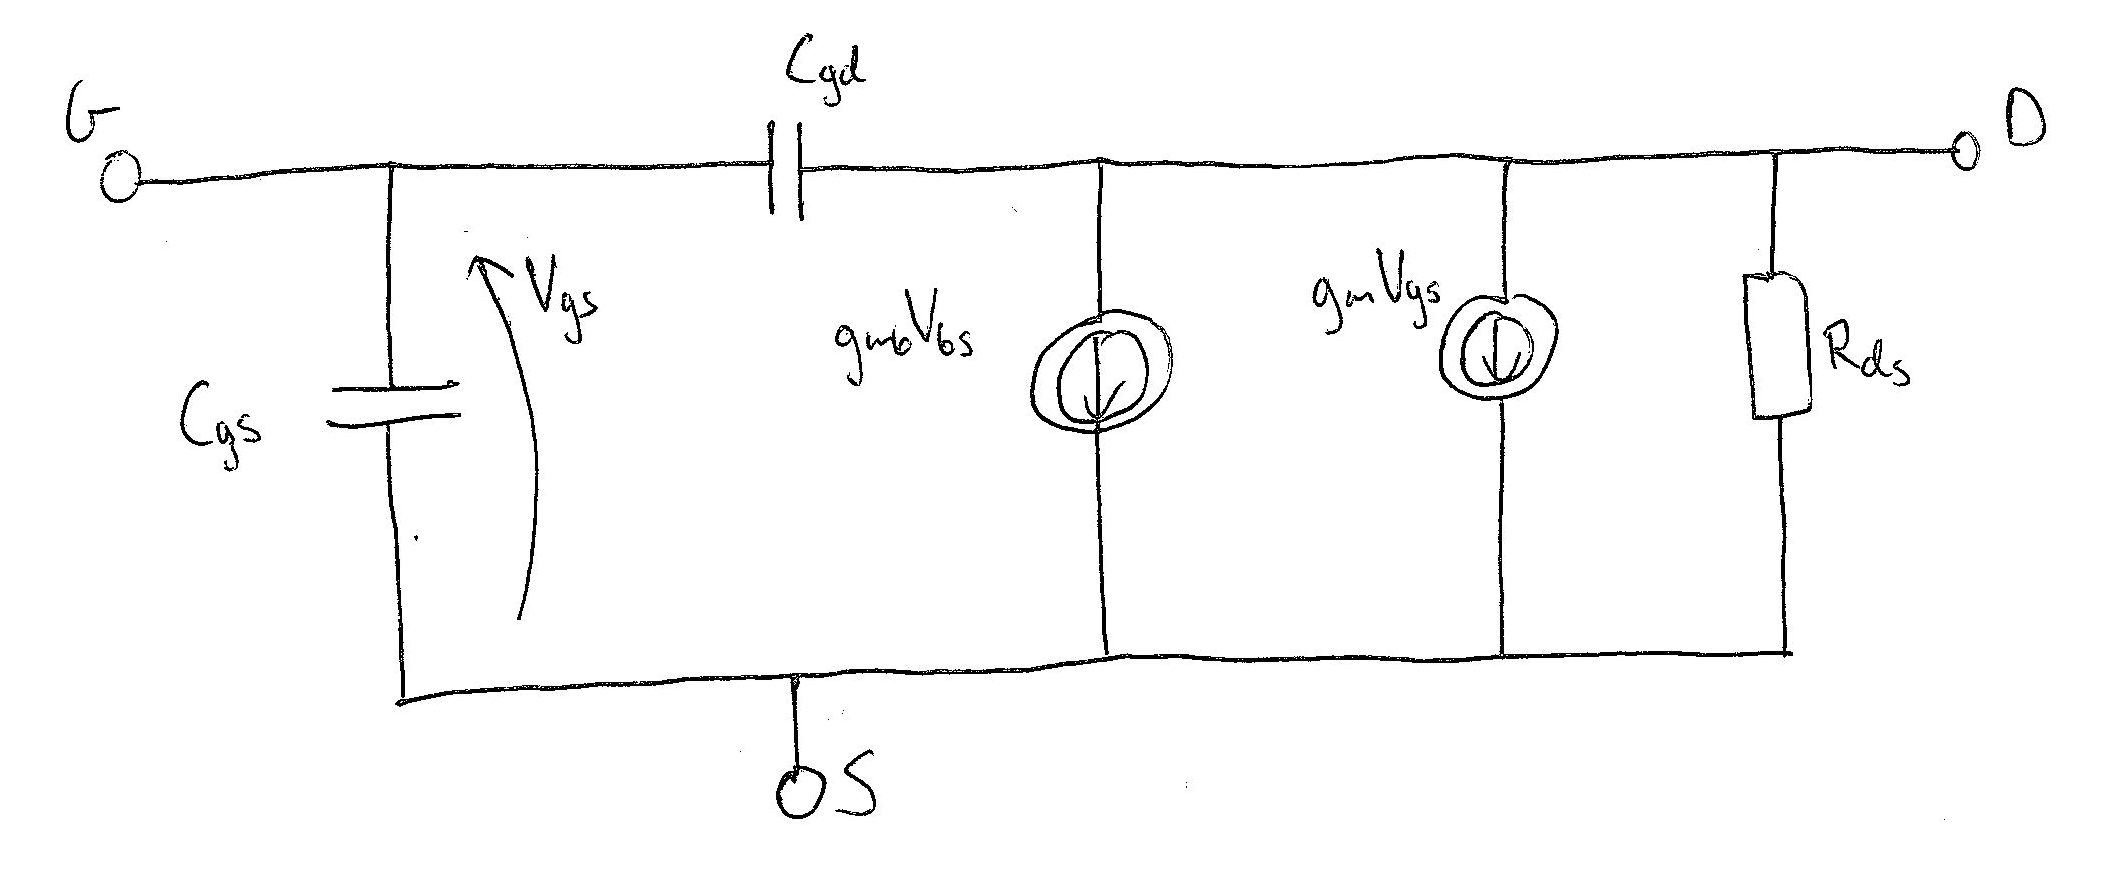
\includegraphics[width=0.7\textwidth]{malosyg_mos.png}
\caption{Charakterystyki wielkosygnałowe}
\end{figure}

\begin{itemize}
\item D - dren
\item G - bramka (Gate)
\item S - źródło (Source) (to ze strzałką na schemacie)
\end{itemize}

\begin{figure}[H]
\centering
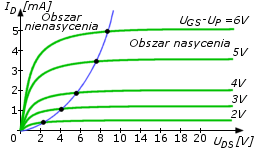
\includegraphics[width=0.5\textwidth]{charPol.png}
\end{figure}

Wykresik podobny do bipolarnego.
\begin{itemize}
\item obszar nienasycenia - triodowy
\item obszar nasycenia - aktywny normalny
\end{itemize}

Tutaj nie ma konkretnego napięcia $V_{TH}$ jak w bipolarnych ($V_{be} = 0.7V$). 

\begin{center}
\begin{tabular}{c|c|c}
& NMOS $V_{TH} > 0$ & PMOS $V_{TH} < 0$ \\
\hline
$V_{GS}$ & $\geq V_{TH}$ & $\leq V_{TH}$ \\ 

$V_{DS}$ & $> V_{GS} - V_{TH}$ & $> V_{GS} - V_{TH}$\\ 
\end{tabular}
\end{center}

$V_{TH}$ to jest namięcie od którego tranzystor polowy zaczyna normalnie działać. Skoro nie ma podanej konkretnej wartości, to pewnie różne tranzystory mają różnie.\\
Nie przepisze wyprowadzenie $g_m$, bo i tak nikt tego nei zapamięta. W każdym razie:
\begin{itemize}
\item wynik jest po pierwiastkiem
\item jest wprost proporcjonalne do szerokości kanału
\item jest przeciwnie proporcjonalne do długości kanału
\end{itemize}
Ta długość i szerokość to już kwestia budowy tranzystorów. Wzmocnienie gorsze niż w bipolarnych, ale jak się bardzo skróci długość(l), to wzmocnienie sie poprawia, a teraz wszystko się skraca, więc polowe są popularne.

\subsection{Luźne uwagi}
\begin{itemize}
\item model wielkosygnałowy jest potrzebny do znalezienia punktu pracy tranzystora(obszaru aktywnego normalnego)
\item w modelu małosygnałowym pojemności są po to, zeby pokazać, ze tranzystor nie działą natychmiastowo
\item duży obwód to emiter-kolektor lub źródło-dren
\item mały obwód (sterujący) to baza-emiter lub -bramka-źródło
\item $g_m$ w bipolarnym zmieni się liniowo, a w polowym jest pod pierwiastkiem, więc ogólnie polowe gorzej wzmacniają
\end{itemize}

\subsection{Wzmocnienie prądowe tranzystora polowego - charakterystyka częstotliwościowa}

\begin{figure}[H]
\centering
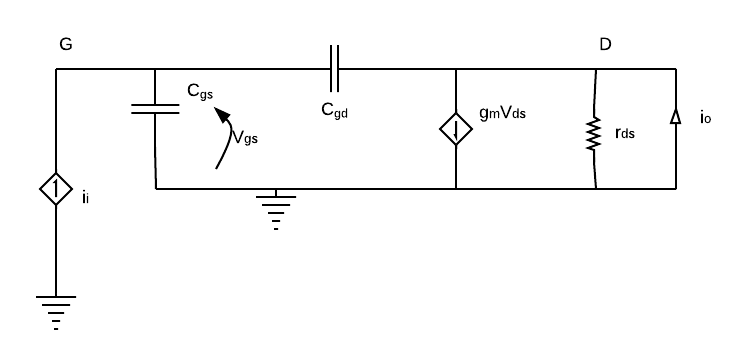
\includegraphics[width=0.7\textwidth]{wzmoc_tranzystora.png}
\end{figure}

Przykłada się $i_i$ i mierzy wzmocnienie prądowe ($\frac{i_o}{i_i}$)\\
\\
R wyjściowe jak najmniejsze, więc jest na końcu zwarcie
\begin{equation}
i_o = g_m V_{gs}
\end{equation}

\begin{equation}
V_{gs} = i_i \frac{1}{s(C_{gs} + C_{gd})}
\end{equation}

\begin{equation}
k_i = \frac{i_o}{i_i} = \frac{ \frac{g_m i_i}{s(C_{gs} + C_{gd})} }{i_i} = \frac{g_m}{s(C_{gs} + C_{gd})}
\end{equation}

\begin{equation}
|k(j\omega)| = \frac{gm}{\omega(C_{gs} + C_{gd})} = 1
\end{equation}

\begin{equation}
\omega _t = \frac{gm}{C_{gs} + C_{gd}}
\end{equation}

$C_{gd}$ - bardzo mała pojemność pasożytnicza więc pozbywamy się
\begin{equation}
\omega _t \approx \frac{gm}{C_{gs}}
\end{equation}

Dla tranzystora bipolarnego wynik analogiczny:
\begin{equation}
\omega _t \approx \frac{gm}{C_{be}}
\end{equation}


\section{Układy jednotranzystorowe}
Układy połączenia dla bipolarnych. Analogicznie robi się dla polowych - po prostu za tranzystor bipolarny wkładamy MOS-a. Schematy są dla npn/nMOS, dla pnp/pMOS robi się tak samo, tylko trzeba pilnować gdzie jest emiter.

Wzmocnienia i w ogóle wszelkie charakterystyki liczymy zastępując tranzystor modelem małosygnałowym (innym dla bipolarnych, innym dla polowych). Z tego już można wyliczyć co trzeba, najwygodniej metodą oczkową. Trzeba uważać na źródła prądowe sterowane.

Ogólna zasada: na jednej nóżce jest sygnał wejściowy, na drugiej wyjściowy, a na trzeciej nóżce nie ma nic i właśnie ta trzecia nóżka jest "wspólna".
\subsection{wspólna bramka (analogicznie wspólna baza)}

\begin{figure}[H]
\centering
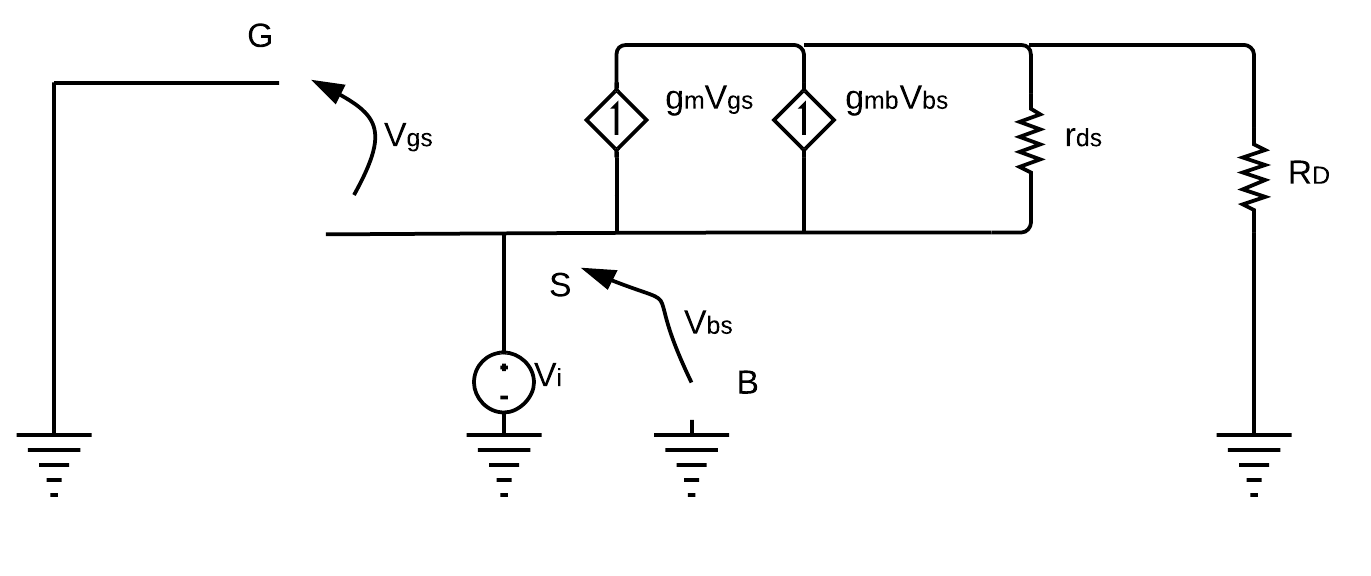
\includegraphics[width=0.5\textwidth]{CG.png}
\end{figure}

\begin{equation}
V_{gs} = -V_i
\end{equation}
\begin{equation}
V_{bs} = -V_i
\end{equation}

\begin{equation}
k_u = {V_o \over V_i}
\end{equation}

\begin{equation}
V_o = I_o R_D
\end{equation}

Tu robimy kilka sztuczek: łączymy źródła prądowe w jedno, potem łączymy to źródło co nam wyszło z opornikiem i z jakiegoś twierdzenia mamy zamiast tego szeregowo połączony opornik ze źródłem napięciowym. Metoda oczkowa z całym jednym oczkiem:

\begin{equation}
[r_{ds} + R_D][i_o]=[V_i - r_{ds}(g_mV_{gs} + g_{mb}V_{bs})]
\end{equation}
Korzystamy z zależności $V_{gs} i V_{bs}$ i mamy:

\begin{equation}
[r_{ds} + R_D][i_o]=[V_i (1 + r_{ds}(g_m + g_{mb}))]
\end{equation}
czyli:\\
\begin{equation}
I_o = {V_i(1+r_{ds}(g_m + g_{mb}))\over r_{ds} + R_D}
\end{equation}

Podstawiamy do wzoru na $k_u$ (skraca się $V_i$ i mnoże przez $R_D$:\\
\begin{equation}
k_u = {(1+r_{ds}(g_m + g_{mb}))R_D\over r_{ds} + R_D}
\end{equation}

To nie koniec! Teraz znowu magia: usuwamy jedynkę! Dzieje się to na pdostawie właściwości tranzystorów:\\
\begin{itemize}
\item bipolarne: ${1 \over g_m }<< r_{be} << r_{ce}$
\item polowe: ${1 \over g_m }<< r_{ds} => 1 << r_{ds}g_m$ (wyżej analogicznie)
\end{itemize}

\begin{equation}
k_u \approx {(g_m + g_{mb})R_Dr_{ds}\over r_{ds} + R_D}
\end{equation}

Te oporności, to wzór na równoległe połączenie, więc można zapisać krócej:

\begin{equation}
k_u \approx {(g_m + g_{mb})R_D || r_{ds}}
\end{equation}

W bipolarnych jest niemalże identycznie, liczy się podobnie, tylko trzeba uwzględnić jeszcze oczko baza-emiter - w polowych nie występuje, bo nie ma połączenia bramka-źródło(w bipolarnych jest tam opornik). Uwzględnienie oporności $r_{be}$ powoduje, że macierz oczkowa jest 2x2! We wzorze ostatecznym różnica to brak $g_{mb}$:

\begin{equation}
k_u = {g_m(R_D || r_{ds})}
\end{equation}

Dalej...

\begin{equation}
r_i = {V_i \over I_i} 
\end{equation}

Podobno $I_i = I_o$, więc:

\begin{equation}
r_i = {V_i(r_{ds} + R_D) \over V_i(1+r_{ds}(g_m + g_{mb}))} \approx {r_{ds} + R_D \over r_{ds}(g_m + g_{mb})}
\end{equation}

Skróciłem $V_i$ i zrobiłem taki sam myk z jedynką co przy $k_u$. Dodatkowo jeśli zachodzi $R_D << r_{ds}$, to:

\begin{equation}
r_i \approx  {1 \over (g_m + g_{mb})}
\end{equation}

Na koniec $r_o$ - liczymy przy wyłączonym $v_i$:\\

\begin{equation}
r_o = {V_o \over I_o} 
\end{equation}

Jak nie ma $V_i$ to nie ma $V_{gs}$ i $V_{bs}$, więc nie działają źródła proądowe. Jak na moje oko wtedy nie ma ani $V_o$ ani $I_o$, ale wychodzi, że:

\begin{equation}
r_o = R_D || r_{ds}
\end{equation}

\begin{figure}[H]
\centering
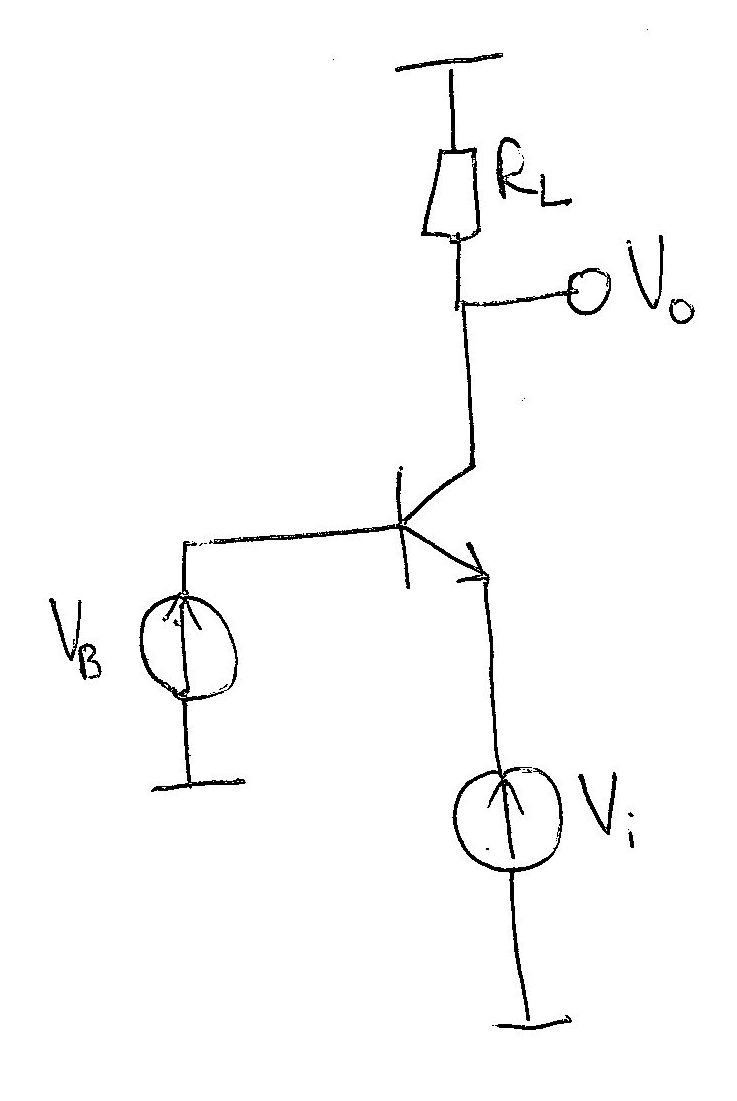
\includegraphics[height=0.3\textwidth]{WB.png}
\begin{tabular}{c|c|c}
& bipolarny & polowy \\
\hline
$r_i$ & $\approx \dfrac{1}{g_m}$ & $ \dfrac{1}{g_m + g_{mb}}$ \\ 

$r_o$ & $r_{ce}\parallel R_C$ & $r_{ds} \parallel R_D $\\ 

$k_u$ & $g_m (r_{ce}\parallel R_C)$ & $(g_m + g_{mb})(r_{ds}\parallel R_D)$  \\ 

$k_i$ & $<1$ & $1$  \\ 

\end{tabular} 
\end{figure}


\textbf{Cechy} (z grubsza dla obu modeli takie same):
\begin{enumerate}
	\item \textbf{$K_u$} duże - dobrze!
	\item \textbf{$r_i$} mała - źle :(
	\item \textbf{$r_o$} duża - źle :(
\end{enumerate}
\textbf{Zastosowania:}
\begin{enumerate}
	\item Są wolne od efektu Millera więc może być wykorzystany we wzmacniaczach wysokiej częstotliwości
\end{enumerate}

\subsection{Wspólne źródło (emiter)}


\begin{figure}[H]
\centering
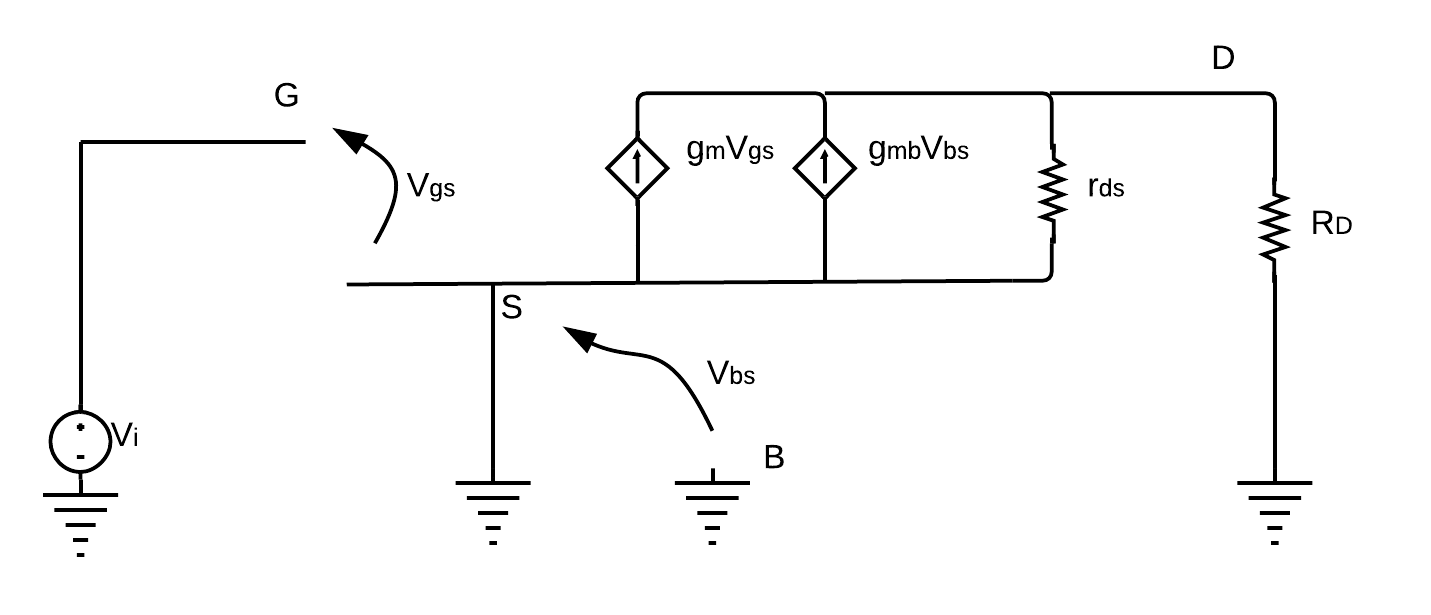
\includegraphics[width=0.5\textwidth]{CS.png}
\end{figure}

$V_{gs} = -V_i$\\
$V_{bs} = 0$ - te same potencjały - odpada jedno źródło prądu\\

\begin{equation}
k_u = {V_o \over V_i}
\end{equation}

\begin{equation}
V_o = -g_mV_i{r_{ds}||R_D}
\end{equation}
Wytłumaczenie: $V_o$ to spadek na $R_D$, $R_D$ połączone równolegle z $r_{ds}$, czyli spadek na nich jest taki sam, czyli prąd (ze źródła prądowego) razy rezystancja zastępcza. Końcowy wynik jest prosty:

\begin{equation}
k_u = -g_m{r_{ds}||R_D}
\end{equation}

Dalej:

\begin{equation}
r_i = {V_i \over I_i} = {V_i \over 0} = \infty
\end{equation}

Wyjaśnienie: brak przepływu prądu pomiędzy bramką, a źródłem dlatego to 0.

\begin{equation}
r_o = R_D || r_{ds}
\end{equation}

Wyjaśnienie - jak przy poprzedniej konfiguracji.

Przy bipolarnym z racji połączenia baza-emiter $r_i = r_{be}$. W pozostałych przypadkach we wzorach zmieniają się tylko literki.

\begin{figure}[H]
\centering
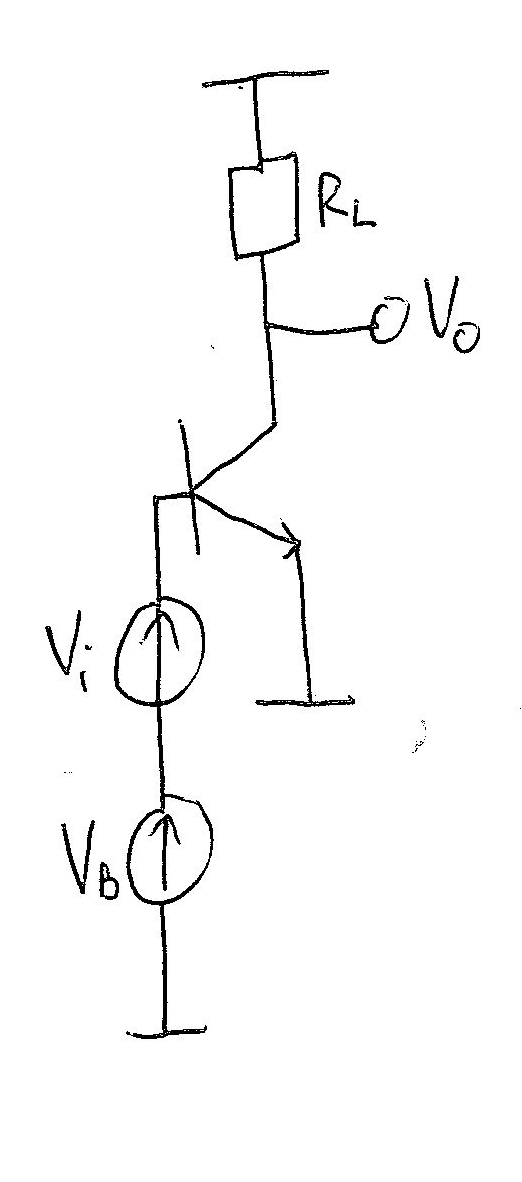
\includegraphics[height=0.3\textwidth]{WE.png}
\begin{tabular}{c|c|c}
& bipolarny & polowy\\
\hline
$r_i$ & $r_{be}=\dfrac{\beta}{g_m}$ & $\infty$ \\ 

$r_o$ & $r_{ce}\parallel R_C$ & $r_{ds} \parallel R_D$\\ 

$k_u$ & $-g_m (r_{ce}\parallel R_C)$ & $-g_m(r_{ds}\parallel R_D)$ \\ 

$k_i$ & $g_m r_{be} = \beta$ & $\infty$ \\ 

\end{tabular} 
\caption{Rysunek wspólnego emitera, ale wystarczy podmienić na MOSa i też będzie}
\end{figure}


\textbf{Cechy} (z grubsza dla obu modeli takie same):
\begin{enumerate}
	\item \textbf{$K_u$} duże - dobrze!
	\item \textbf{$r_i$} duża - dobrze!
	\item \textbf{$r_o$} duża - źle :(
\end{enumerate}
\textbf{Zastosowania:}
\begin{enumerate}
	\item Często jako wzmacniacz napięcia, szczególnie w zakresie niezbyt wysokich częstotliwości granicznych
\end{enumerate}

\subsection{Wspólny dren (kolektor)}


\begin{figure}[H]
\centering
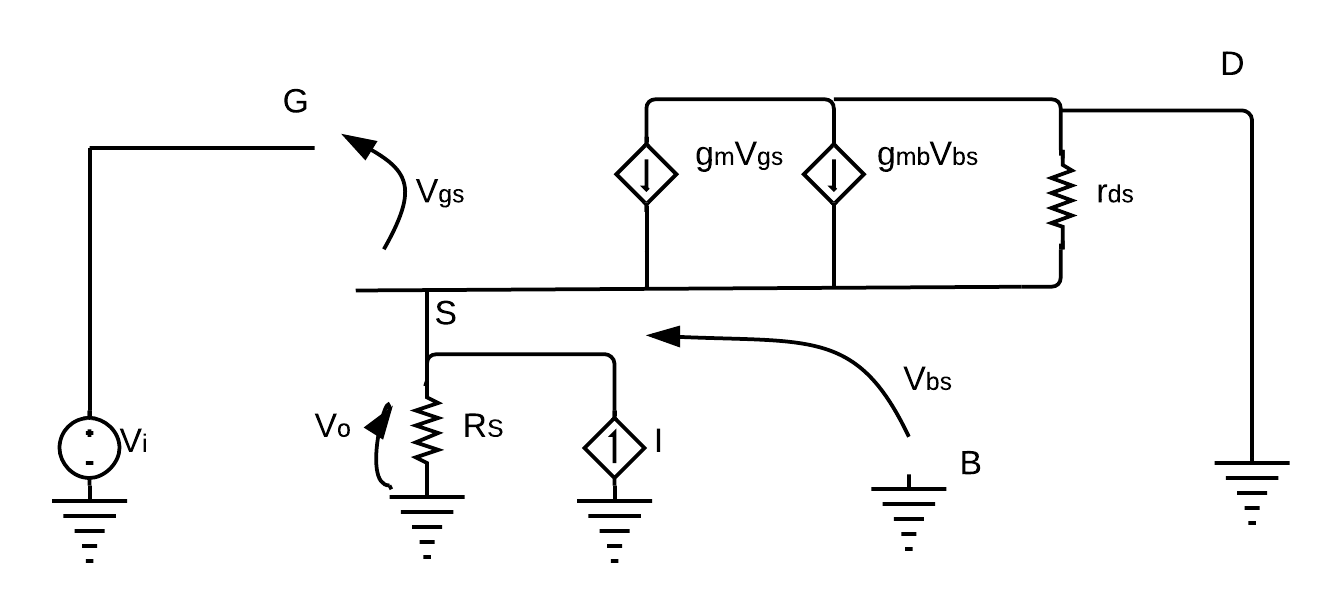
\includegraphics[width=0.5\textwidth]{CD.png}
\end{figure}

\begin{equation}
k_u = {V_o \over V_i}
\end{equation}

$V_o$ - spadek na $R_S$. $R_S$ połączone równolegle z $r_{ds}$ - robimy zastępczą. Płynie przez nie prąd z obu źródeł prądowych, więc mamy taki wynik:

\begin{equation}
V_o = {(g_mV_{gs} + g_{mb}V_{bs})(R_S || r_{ds})}
\end{equation}

(Powyższe można też obliczyć metodą węzłową.
\begin{equation}
V_gs = V_i - V_o
\end{equation}
\begin{equation}
V_bs = - V_o
\end{equation}

\begin{equation}
V_o = {(g_mV_i - g_mV_o - g_{mb}V_{o})(R_S || r_{ds})}
\end{equation}

\begin{equation}
{V_o \over R_S || r_{ds}} + g_mV_o + g_{mb}V_{o}= {g_mV_i }
\end{equation}

\begin{equation}
{V_o ({1\over R_S || r_{ds}} + g_m + g_{mb})= g_mV_i }
\end{equation}

Teraz trzeba do wspólnego mianownika nawias z lewej strony i wywalić go na prawą. Pozwolę sobie opuścić to. 

\begin{equation}
V_o = {V_ig_m(R_S || r_{ds}) \over (g_m + g_{mb})r_{ds}||R_s + 1}
\end{equation}
To jest inaczej niż w notatkach Sylwii, ale śmiem twierdzić, ze mam racje, bo zgadza się to z tym, co potem pisze o $k_u$:P

\begin{equation}
k_u = {V_o \over V_i} = {g_m(R_S || r_{ds}) \over (g_m + g_{mb})r_{ds}||R_s + 1} \approx = {g_m(R_S || r_{ds}) \over (g_m + g_{mb})(r_{ds}||R_s)} \leq 1
\end{equation}

Znowu w jakiś magiczny sposób znika nam jedynka (bo jest dużo mniejsza od tego iloczynu koło niej), i tak koniec końców dowiadujemy się, że to jest nie większe od 1 (co wynika ze wzoru w sumie).

\begin{equation}
r_i = {V_i \over I_i} = {V_i \over 0} = \infty
\end{equation}

Wytłumaczenie tak jak wyżej. 

\begin{equation}
r_o = {V_o \over I_o}
\end{equation}

Tutaj znowu jakieś cuda... Tzn. bardzo banalne rzeczy (ew. jak powiedział keidyś prof. Idzik 'to jest proste, ale nie banalne'). Zwieramy $V_i$ (jak zawsze przy liczeniu $r_o$) i dodajemy źródło prądu $I$ między masą, a potencjałem $V_o$.

\begin{figure}[H]
\centering
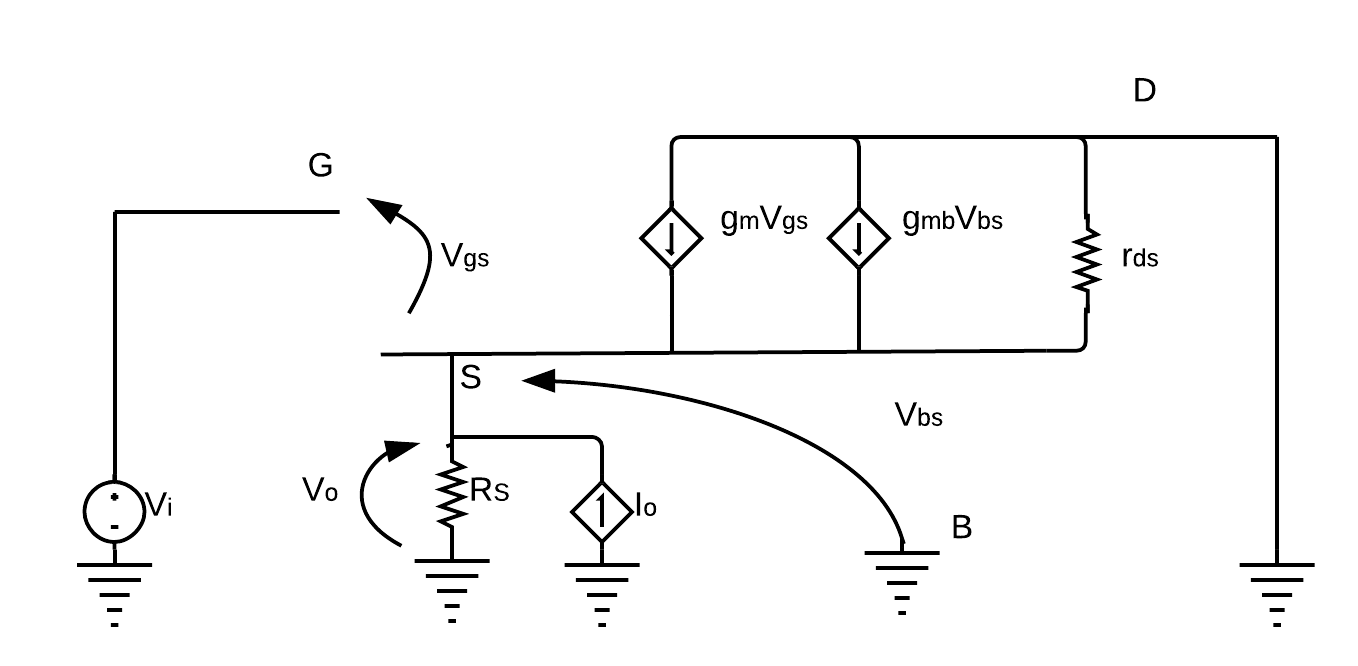
\includegraphics[width=0.5\textwidth]{CD2.png}
\end{figure}

Wtedy otrzymujemy:
\begin{equation}
V_gs = - V_o
\end{equation}
\begin{equation}
V_bs = - V_o
\end{equation}

Układ jak go sobie ładnie narysujemy, to równoległe połączenie 2 oporników i 3 źródeł prądowych. więc jak połączymy źródła i oporniki otrzymujemy:

\begin{equation}
V_o = {I_z R_z} = (I + g_mV_{gs} + g_{mb}V_{bs})(R_S || r_ds) = (I - g_mV_o - g_{mb}V_o)(R_S || r_ds) = (I - V_o(g_m + g_{mb}))(R_S || r_ds)
\end{equation}

\begin{equation}
I = {V_o \over R_S || r_ds} + V_o(g_m + g_{mb}) = V_o\left({1 \over R_S || r_ds} + g_m + g_{mb}\right)
\end{equation}

$I$ jest w sumie równoważne $I_o$, więc:

\begin{equation}
r_o = {V_o \over I_o} = {1 \over{1 \over R_S || r_ds} + g_m + g_{mb}} \approx {1 \over g_m + g_{mb}}
\end{equation}

\begin{figure}[H]
\centering
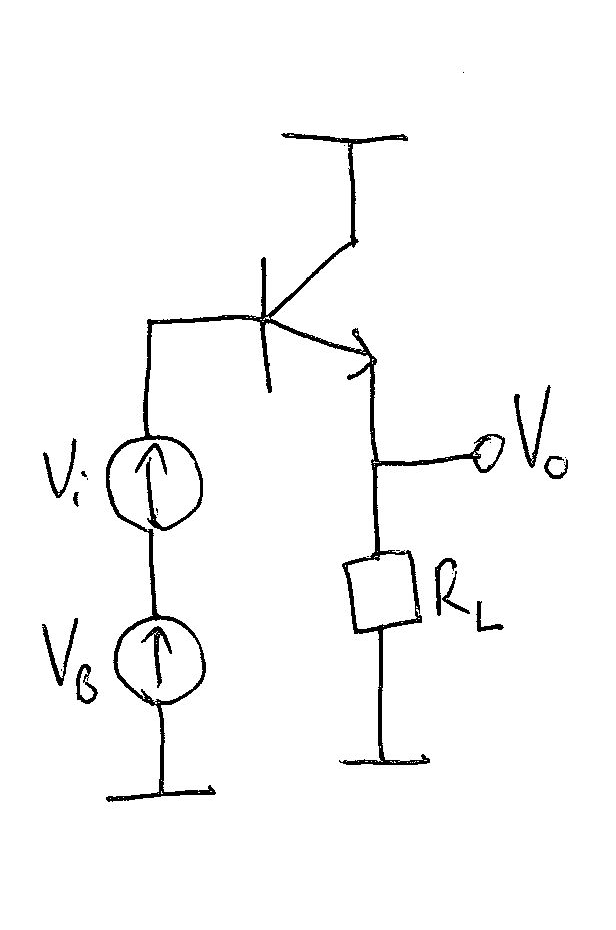
\includegraphics[height=0.3\textwidth]{WC.png}
\begin{tabular}{c|c|c}
& bipolarny & polowy\\
\hline
$r_i$ & $r_{be} + \beta R_E$ & $\infty$ \\ 

$r_o$ & $\dfrac{1}{\dfrac{1}{r_{be}}+\dfrac{1}{R_E}+\dfrac{1}{r_{ec}}+g_m}$ & $\dfrac{1}{g_m + g_{mb}}$ \\ 

$k_u$ & $\dfrac{g_m}{g_m+\dfrac{1}{R_E}}$ & $\dfrac{g_m}{g_m+g_{mb}}$ \\ 

$k_i$ & $g_m r_{be} = \beta$ & $\infty$ \\ 

\end{tabular} 
\end{figure}


\textbf{Cechy} (z grubsza dla obu modeli takie same):
\begin{enumerate}
	\item \textbf{$K_u$} małe - źle :(
	\item \textbf{$r_i$} duża - dobrze!
	\item \textbf{$r_o$} mała - dobrze!
\end{enumerate}
\textbf{Zastosowania:}
\begin{enumerate}
	\item Wysokie wzmocnienie prądowe - wykorzystywany tam gdzie potrzeba wysterowania następnych stopni wzmacniacza wymagających stosunkowo dużego sygnału prądowego
	\item Jako stopień separujący
\end{enumerate}


\subsection{Zdegenerowane źródło(emiter)}


\begin{figure}[H]
\centering
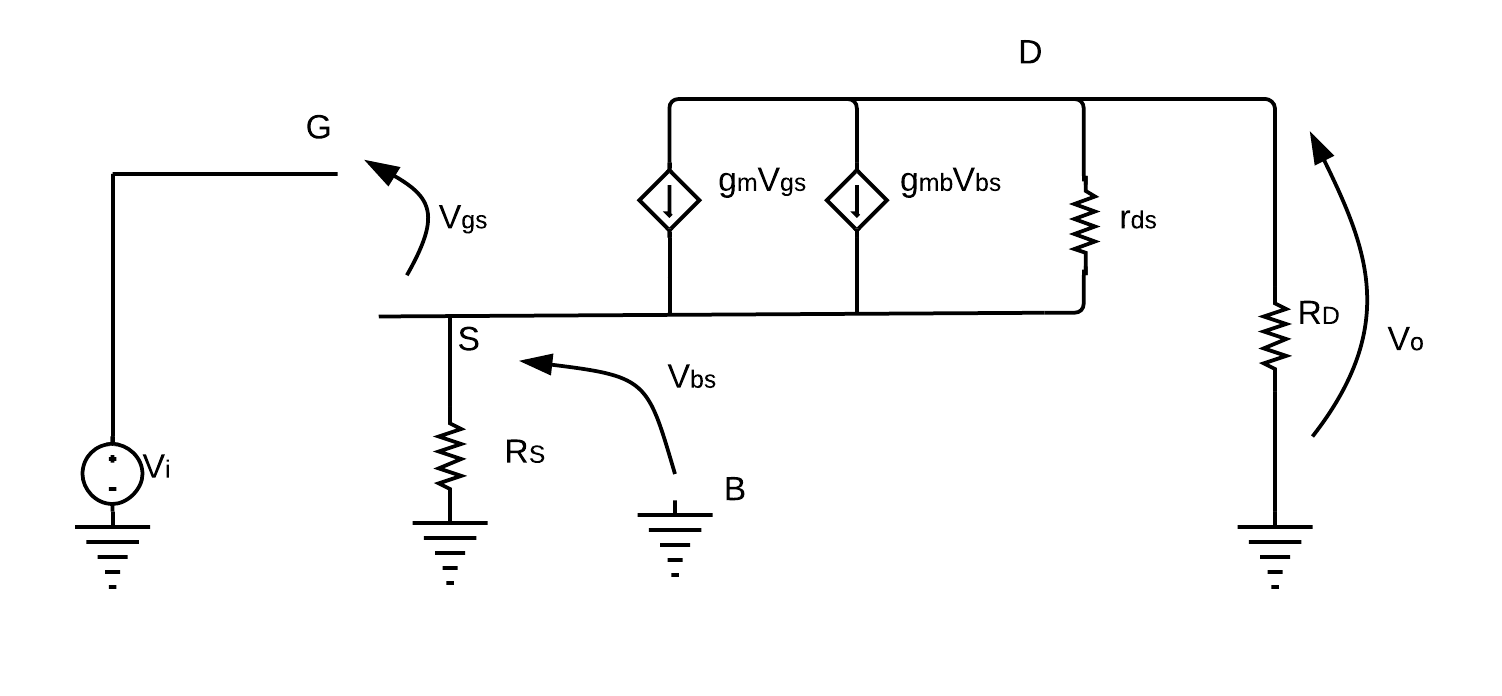
\includegraphics[width=0.5\textwidth]{DS.png}
\end{figure}

\begin{equation}
V_{gs} = V_i + i_0R_S 
\end{equation}

\begin{equation}
V_{bs} = i_0R_S
\end{equation}

\begin{equation}
k_u = {V_o \over V_i}
\end{equation}

\begin{equation}
v_o = i_0R_D
\end{equation}

Teraz tak:
\begin{itemize}
\item łączymy źródła prądowe w jedno
\item z tw. Thevenina (lub Nortona, nie pamiętam) zmieniamy powstałe źródło prądowe i $r_{rs}$ (równoległe) w szeregowe połączenie źródła napięciowego i tejże oporności
\end{itemize}
Otrzymujemy jedno oczko z trzema opornościami i źródłem napięciowym. Zapisujemy równanie:

\begin{equation}
i_o = {R_z \over U} = { -(gmV_{gs} + g_{mb}V_{bs})r_{ds} \over R_S + r_{ds} + R_D} = -{g_mV_ir_{ds} \over R_S + r_{ds} + R_D + (g_m+g_{mb})r_{ds}R_S} \approx -{g_mV_i \over  (g_m+g_{mb})R_S} 
\end{equation}

Jest trochę tych przekształceń, ale rzeczywiście wynik się zgadza:) $V_{gs}$ i $V_{bs}$ standardowo podstawione. Potem standardowa seria przybliżeń, kótre mówią same za siebie: 
\begin{equation}
 R_S + r_{ds} + R_D << (g_m+g_{mb})r_{ds}R_S
\end{equation}
A $r_{ds}$ się skróciło.

\begin{equation}
k_u = {V_o \over V_i} \approx -{g_mV_iR_D \over  V_i(g_m+g_{mb})R_S} = -{g_mR_D \over  (g_m+g_{mb})R_S}
\end{equation}

Tutaj będzie takie przybliżenie od siekiery, ale niech będzie: $g_{mb} = (od 0.1 do 0.3) g_m$, czyli $g_{mb} << g_m$.

\begin{equation}
k_u =-{ R_D \over R_S}
\end{equation}

To w sumie niepotrzebne:
\begin{equation}
r_i = {V_i \over I_i} = {V_i \over 0} = \infty
\end{equation}

$r_o$ nie było na wykładzie, zlitował się.


\begin{figure}[H]
\centering
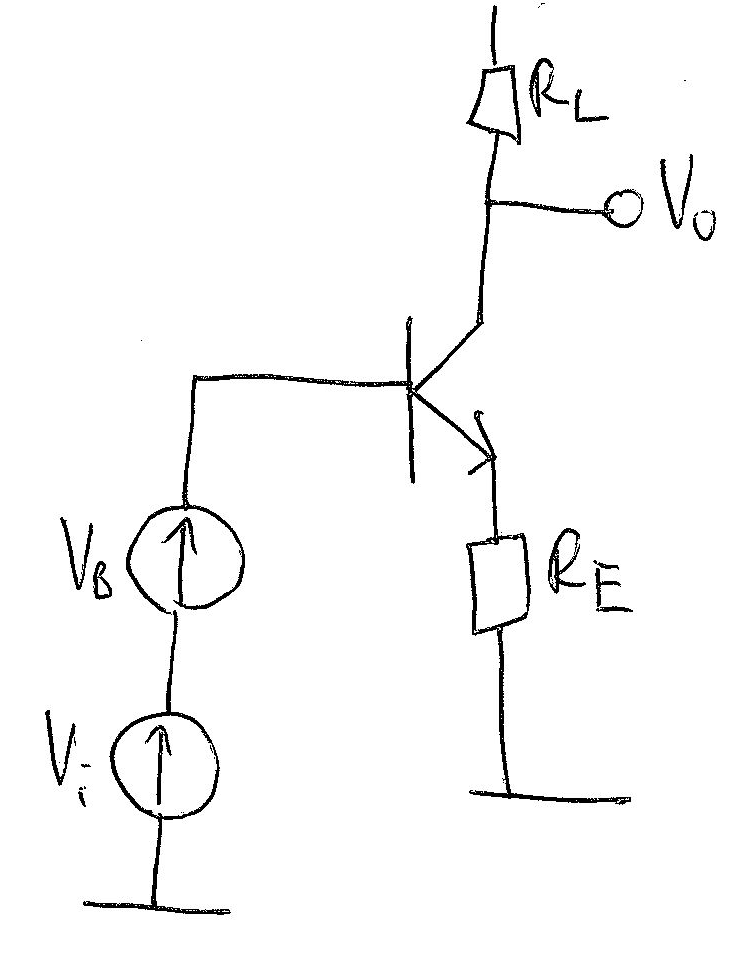
\includegraphics[height=0.3\textwidth]{WDE.png}
\begin{tabular}{c|c|c}
& bipolarny & polowy\\
\hline
$r_i$ & $r_{be} + \beta R_E$ & $\infty$ \\ 

$r_o$ & $\dfrac{1}{\dfrac{1}{r_{be}}+\dfrac{1}{R_E}+\dfrac{1}{r_{ec}}+g_m}$ & $\dfrac{1}{g_m + g_{mb}}$ \\ 

$k_u$ & $-\dfrac{R_C}{R_E}$ & $-\dfrac{R_D}{R_S}$ \\ 

$k_i$ & $?$ & $\infty$ \\ 

\end{tabular} 
\end{figure}


\section{Źródła prądowe}
Służą do:
\begin{itemize}
\item{polaryzacji}
\item{jako aktywne obciążenia}
\end{itemize}
\textbf{Wszystkie poniższe schematy można zrobić też na tranzystorach bipolarnych.}

\subsection{Bufor(?)}

\subsection{Lustro prądowe}
\begin{figure}[H]
\centering
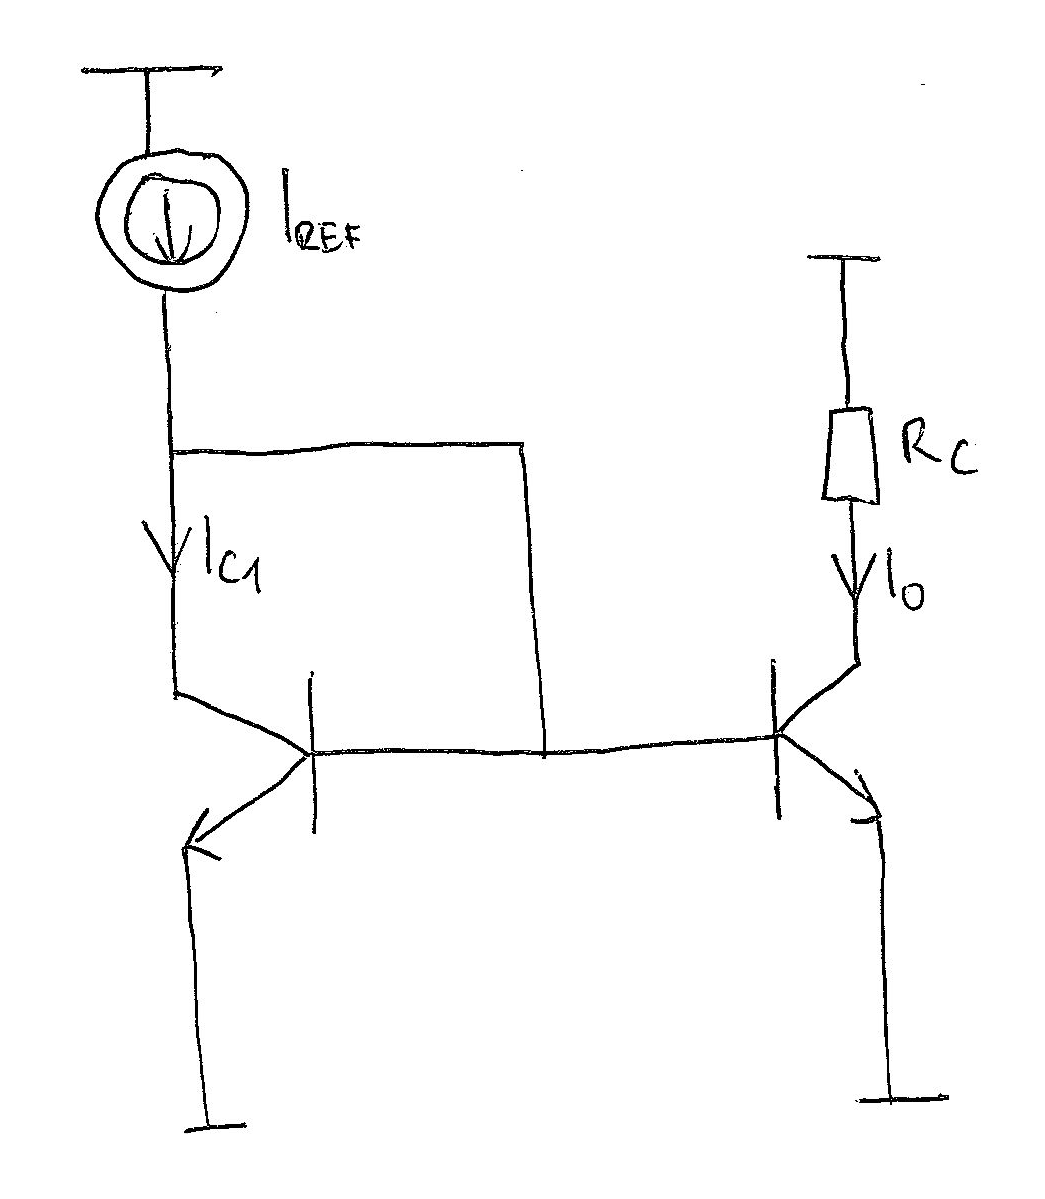
\includegraphics[width=0.35\textwidth]{lustro.png}
\end{figure}
\begin{align*}
I_{REF}&=I_{C1}+2I_B=I_{C1}+\dfrac{2I_{C1}}{\beta}=I(1+\dfrac{2}{\beta}) \\
\dfrac{I}{I_{REF}}&=\dfrac{1}{1+\dfrac{2}{\beta}}
\end{align*}

Model małosygnałowy lustra dla tranzystorów polowych (uwaga: nie powinno być na schemacie źródła prądowego $I_{REF}$ EDIT: $I_{REF}$ oznacza jakąś wartość prądu, która będzie powielana na sąsiedniej stronie lustra. Robi się ją dając jakieś napięcie i opornik):
\begin{figure}[H]
\centering
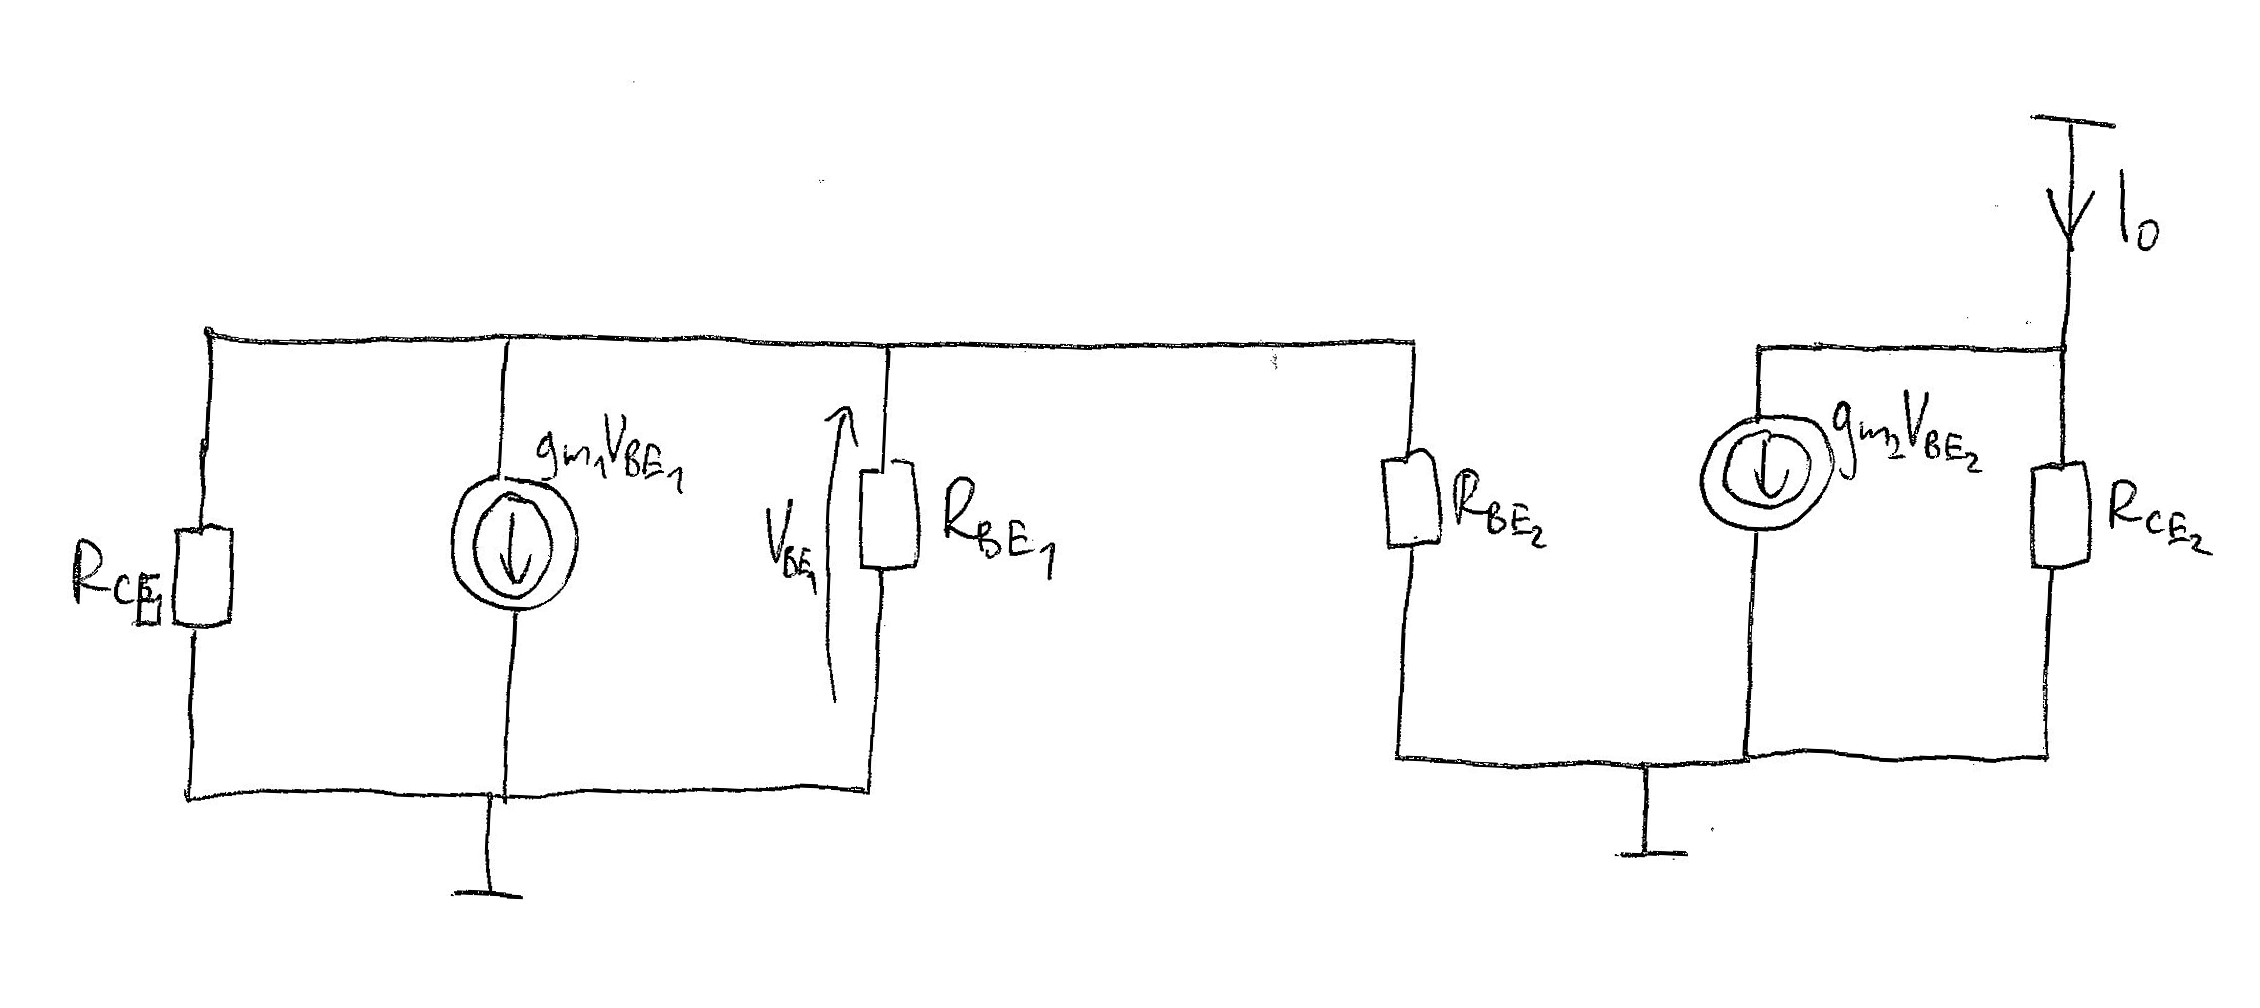
\includegraphics[width=0.5\textwidth]{lustr_wyp1.png}
\end{figure}

Źródeł prądowych $V_{bs}g_{mb}$ nie ma, bo źródło jest na masie, więc $V_{bs} = 0$.

Ze względu na zwarcie przy pierwszym tranzystorze napięcie na gałęzi ze źródłem sterowanym wynosi $V_{gs1}$. Możemy więc policzyć rezystancję na tej gałęzi:
\begin{equation}
r_z = {U \over I} = {V_{gs1} \over V_{gs1}g_m} = {1 \over g_m}
\end{equation}
Czyli zastępujemy to źródło rezystancją:
\begin{figure}[H]
\centering
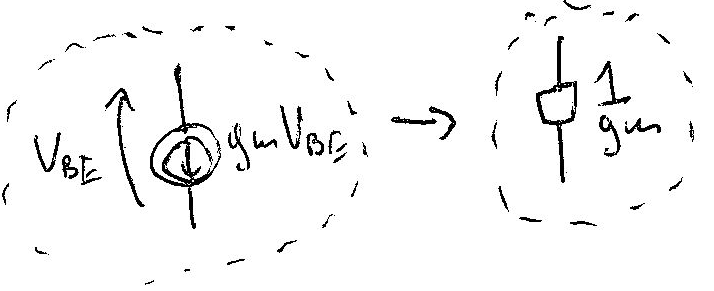
\includegraphics[width=0.35\textwidth]{lustr_wyp2.png}
\end{figure}

Nie wiadomo dlaczego drugie źródło jest równe 0 (prawdopodobnie te dwa źródła prądowe się w praktyce znoszą, a tylko jedno działa jak rezystancja, bo jest na nim napięcie), w każdym razie schemat wygląda teraz tak:
\begin{figure}[H]
\centering
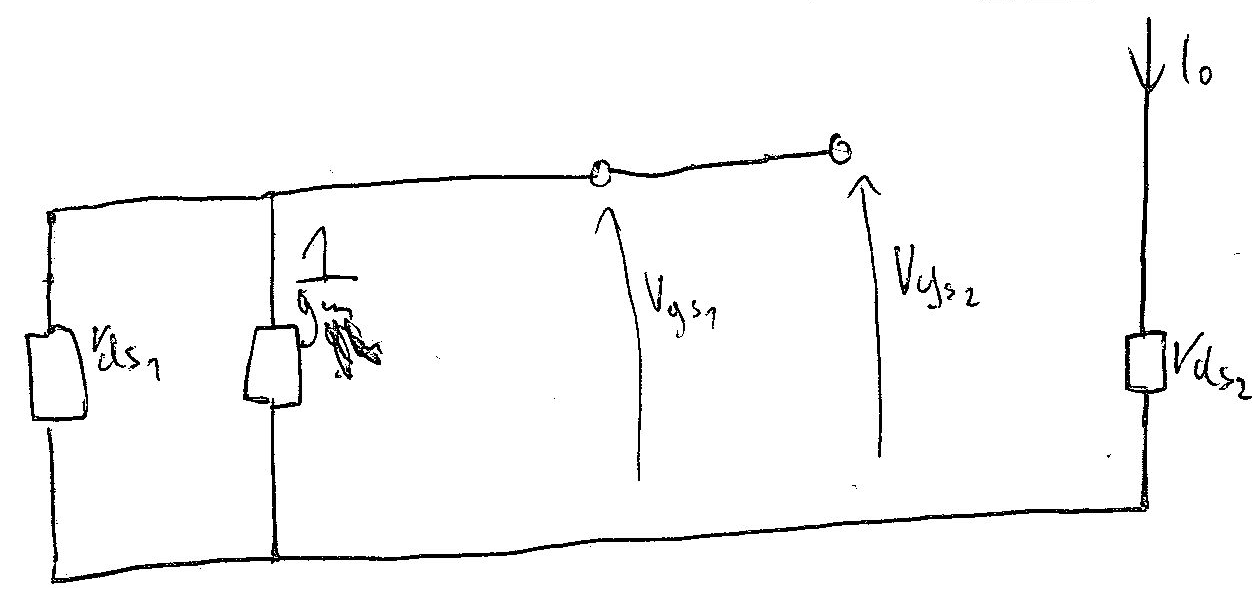
\includegraphics[width=0.45\textwidth]{lustr_wyp3.png}
\end{figure}

Rezystancja wyjściowa: 
\begin{equation}
r_o = \dfrac{V}{I} = r_{ds2}
\end{equation}

\subsection{Kaskodowe źródło prądowe}
\begin{figure}[H]
\centering
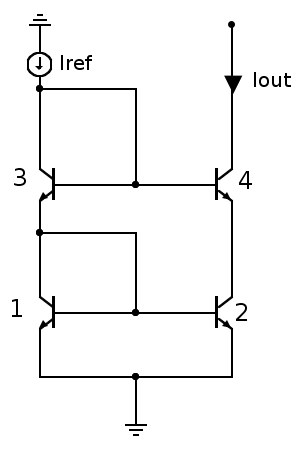
\includegraphics[width=0.3\textwidth]{kaskoda.png}
\end{figure}

Model małosygnałowy kaskody dla polowych (gałąź z $1/g_{m}$ robi się analogicznie jak w lustrze):
\begin{figure}[H]
\centering
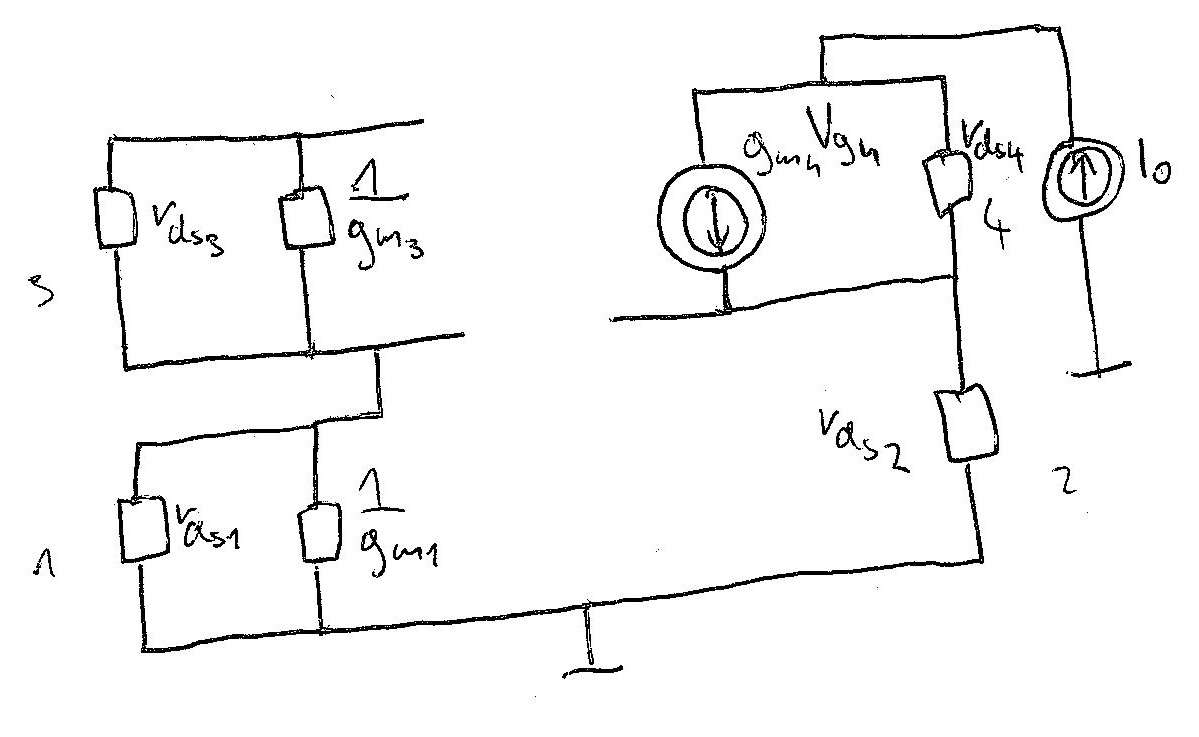
\includegraphics[width=0.5\textwidth]{kaskoda_wypr.png}
\end{figure}
\begin{align*}
U&=(I_o-g_{m4}V_{gs4})r_{ds4}+I_o r_{ds2} \\
V_{gs4}&=-I_o r_{ds2} \\
U&=I_o(r_{ds4}+g_{m4}r_{ds4}r_{ds2}+r_{ds2} \\
r_{out}&=\dfrac{U}{I}=g_{m4}r_{ds4}r_{ds2}+r_{ds4}+r_{ds2}
\end{align*}

\subsection{Różne}
\subsubsection{Zastosowania - Aktywne obciążenia}
Po prostu zastępujemy opornik źródłem prądowym.
\begin{figure}[H]
\centering
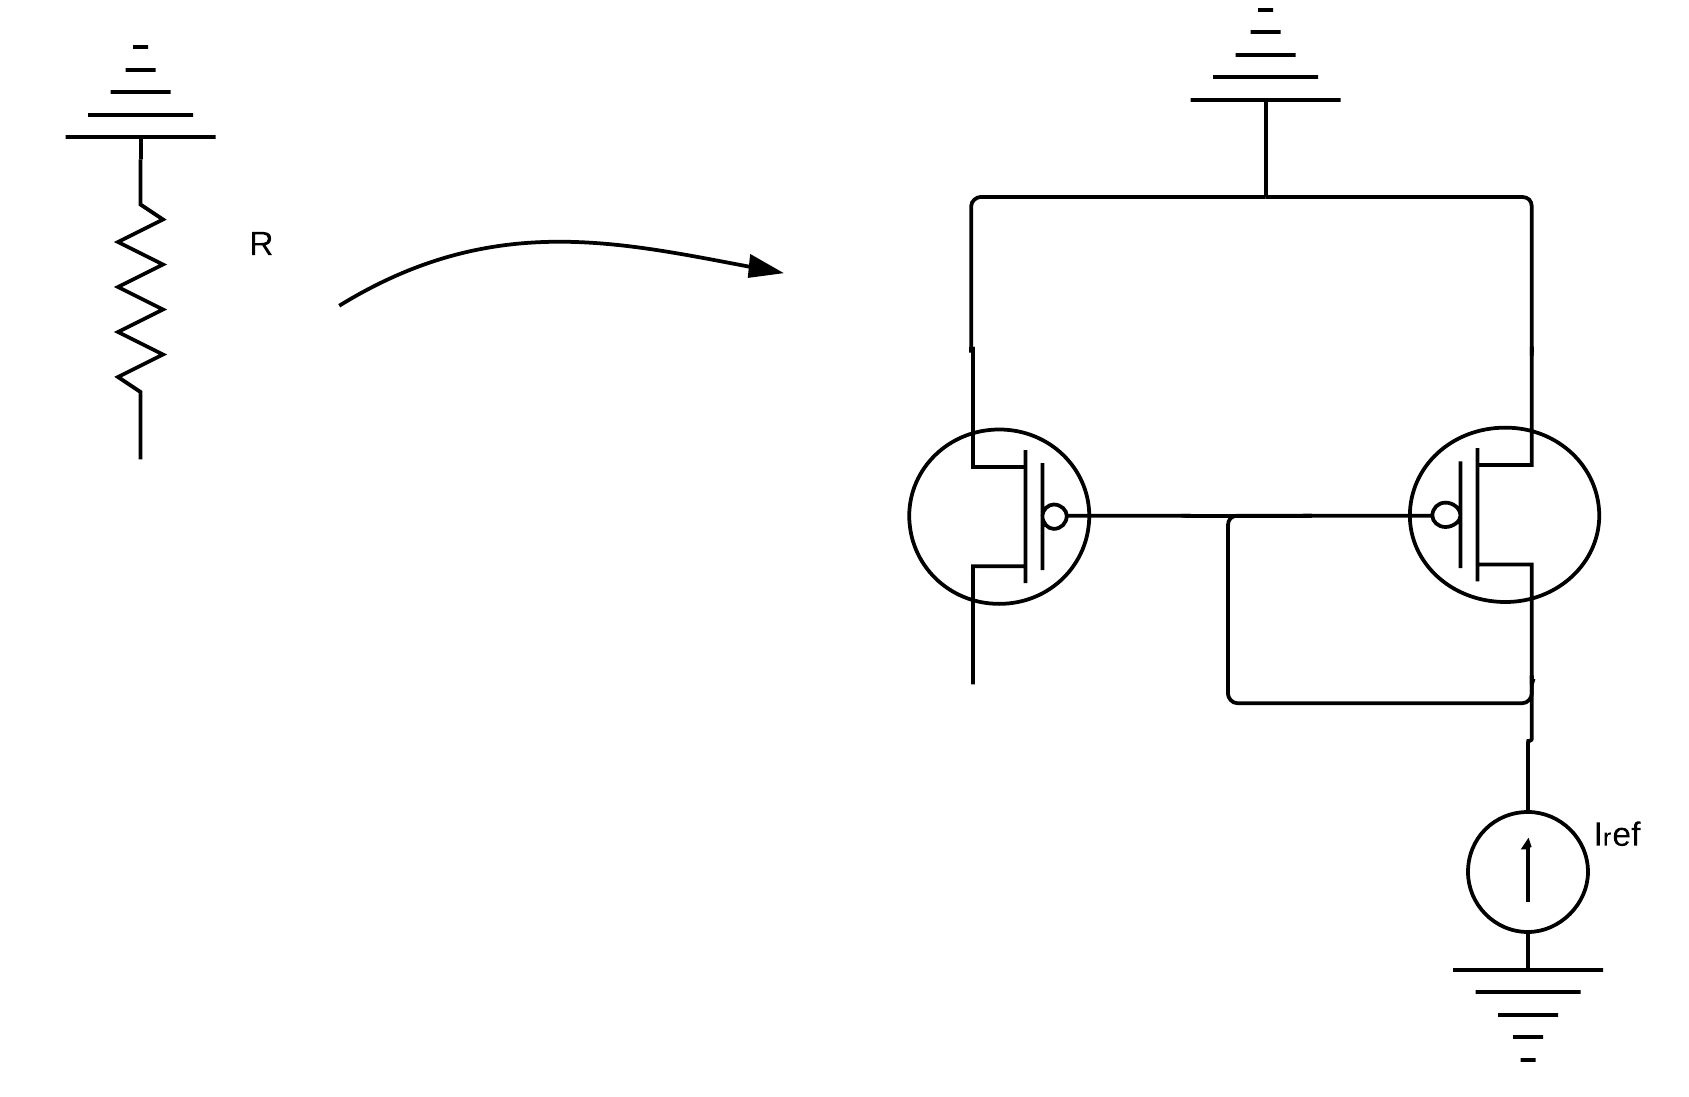
\includegraphics[width=0.5\textwidth]{lustroZast}
\end{figure}
Kółeczka, czyli prąd idzie do tranzystora (PMOS). Chyba. Rezystancja to $r_{ds} \approx 100k \Omega$, czyli dużo 

\subsubsection{Rodzaje - source i sink}
Sink to źródła na NMOSach - wciągają prąd, source to źródła na PMOSach - wynika, że wypuszczają prąd.

\section{Wzmacniacze mocy}
\subsection{Klasa A}
\begin{figure}[H]
\centering
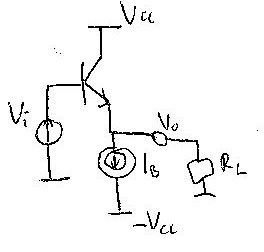
\includegraphics[width=0.3\textwidth]{wzm_moc_a.png}
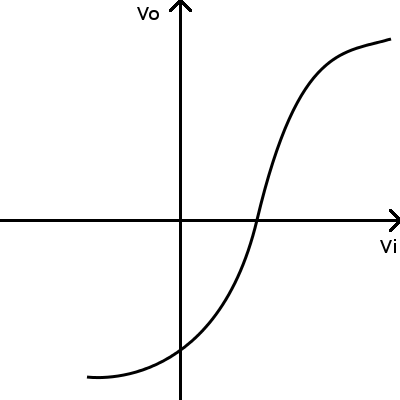
\includegraphics[width=0.3\textwidth]{wzm_moc_a_wyk.png}
\end{figure}
\begin{itemize}
\item{Najprostszy wzmacniacz mocy}
\item{Wykorzystywany zwykle jako bufor}
\item{Najgorsza sprawność}
\item{Używany tylko wtedy, kiedy potrzebna jest liniowość}
\end{itemize}
\begin{align*}
V_i &= V_{BE}+V_O \\
V_O&=V_i-V_{BE} \\
I_C&=I_S e^{\dfrac{V_{BE}}{V_T}} \\
V_O &= V_i -V_T \ln \dfrac{I_C}{I_S} \approx V_i - V_T \ln \dfrac{I_B + \dfrac{V_O}{R_L}}{I_S}
\end{align*}

Sprawność:
\begin{align*}
\eta &= \dfrac{P_L}{P_{total}}\\
P_L &= \dfrac{1}{2\pi} \int \limits^{2 \pi}_{0} V(t)I(t)d\phi = \dfrac{1}{2 \pi} \int \limits^{2 \pi}_{0} V_o \sin \phi \dfrac{V_o \sin \phi}{R_L} d\phi = \dfrac{V_o^2}{2 \pi R_L} \int \limits^{2 \pi}_{0} \sin^2 \phi d\phi = \dfrac{1}{2}\dfrac{V_o^2}{R_L} \\
P_{total} &= 2 V_{cc} I_B \\
\eta &= \dfrac{\dfrac{1}{2} \dfrac{V_o^2}{R_L}}{2 V_{cc} I_B} = \dfrac{V_o \dfrac{V_o}{R_L}}{4 V_{cc} I_B} \\
\end{align*}
\begin{equation}
max(V_o)\rightarrow V_{cc}, max(\dfrac{V_O}{R_L})\rightarrow I_B \quad \rightarrow \quad \eta_{max} < 25\% \nonumber
\end{equation}

\subsection{Klasa B}
\begin{figure}[H]
\centering
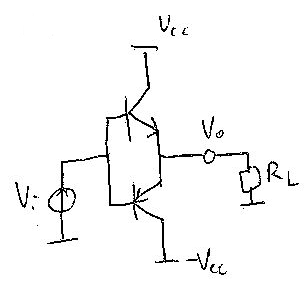
\includegraphics[width=0.3\textwidth]{wzm_moc_b.png}
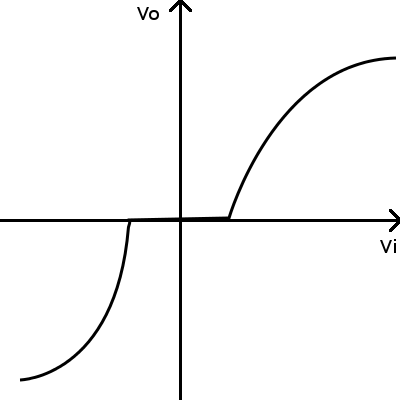
\includegraphics[width=0.3\textwidth]{wzm_moc_b_wyk.png}
\end{figure}
\begin{itemize}
\item{Nie pobiera mocy w stanie statycznym}
\item{Przy wysokim sygnale prąd płynie przez górny tranzystor, przy niskim przez dolny}
\item{liniowość gorsza niż klasy A}
\end{itemize}

Sprawność:
$P_L$ jak poprzednio. $P_{total}$ liczymy tylko od $0$ do $\pi$, bo w drugiej połowie okresu moc jest taka sama.
\begin{align*}
P_{total} &= \dfrac{1}{\pi} \int \limits^\pi_0 V_{cc} \dfrac{V_o \sin \phi}{R_L} d\phi = \dfrac{2 V_{cc} V_o}{\pi R_L}\\
\eta &= \dfrac{\dfrac{V_o^2}{2 R_L}}{\dfrac{2 V_{cc} V_o}{\pi R_L}} = \dfrac{\pi V_o}{4 V_{cc}}\\
\end{align*}
\begin{equation}
\eta_{max} < \dfrac{\pi}{4} \approx 78,6\%
\end{equation}

\subsection{Klasa AB}
\begin{figure}[H]
\centering
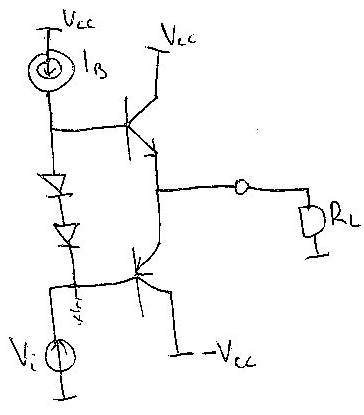
\includegraphics[width=0.3\textwidth]{wzm_moc_ab.png}
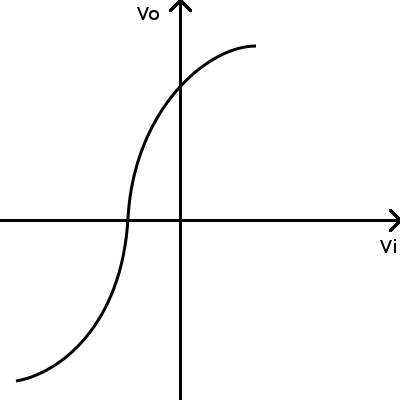
\includegraphics[width=0.3\textwidth]{wzm_moc_ab_wyk.png}
\end{figure}
\begin{itemize}
\item{Energia tracona na tranzystorach}
\item{Przy małych sygnałach przewodzą oba tranzystory (praca w klasie A) przy dużych jeden (praca w klasie B)}
\item{Powszechnie stosowany w audio}
\end{itemize}

\subsection{Klasa D}
\begin{figure}[H]
\centering
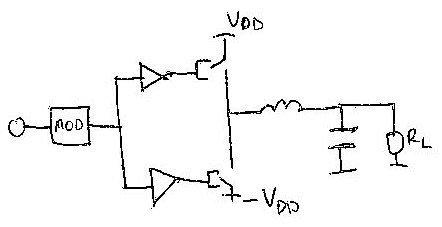
\includegraphics[width=0.5\textwidth]{wzm_moc_d.png}
\end{figure}
\begin{itemize}
\item{Tranzystory działają jak klucz}
\item{W idealnym przypadku $\eta \rightarrow 100\%$}
\item{Sygnał jest przerabiany na sygnał prostokątny, po wzmocnieniu puszczony przez filtr dolnoprzepustowy (cewka zamiast wzmacniacza, żeby nie tracić mocy)}
\end{itemize}

\section{Wzmacniacze różnicowe}
Właściwości:
\begin{itemize}
\item{Eliminuje zakłócenia wspólne i te od zasilania}
\item{Amplituda 2x większa}
\item{Łatwa polaryzacja}
\end{itemize}
\begin{figure}[H]
\centering
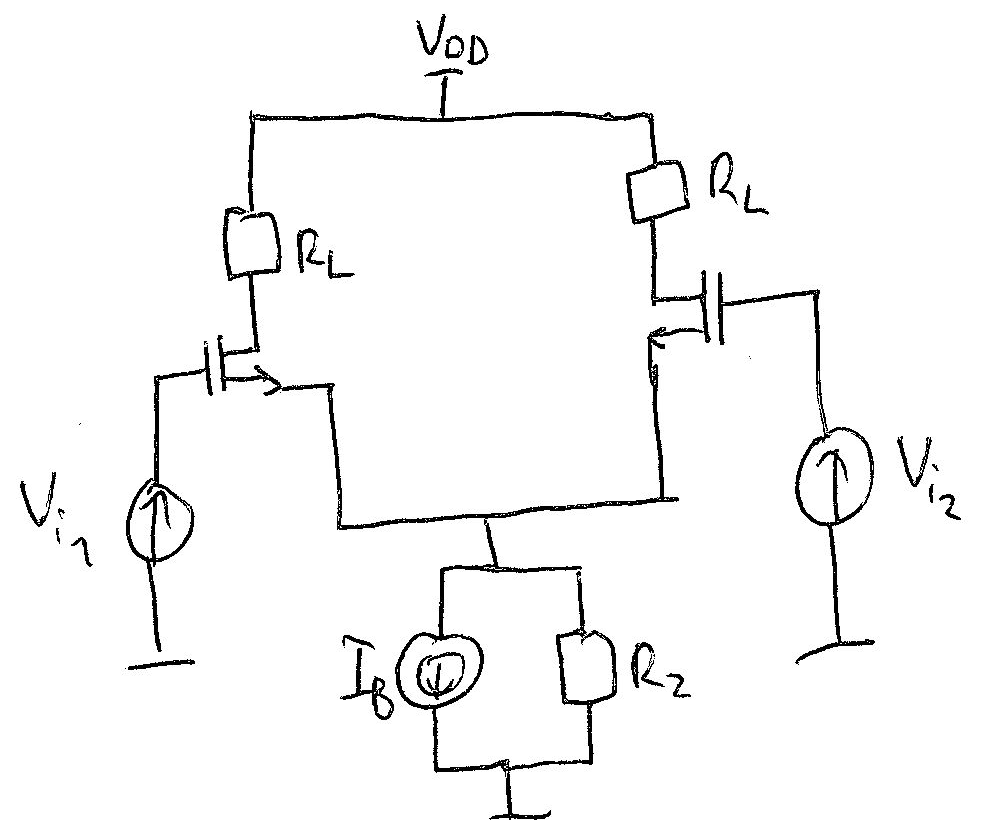
\includegraphics[width=0.4\textwidth]{roznicowy.png}
\end{figure}

\subsection{Analiza małosygnałowa}

Definiujemy nową, wspólną zmienną na wejściu:
\begin{equation}
v_{id}=v_{i1}-v_{i2}
\end{equation}

Średnią napięcia wejściowego definiujemy następująco: $v_{ic}=\dfrac{v_{i1}+v_{i2}}{2}$. Przekształcamy, żeby uzyskać napięcia wejściowe zależne od $v_{id}$ i $v_{ic}$:
\begin{align*}
v_{i1}&=v_{ic}+\dfrac{v_{id}}{2} \\
v_{i2}&=v_{ic}-\dfrac{v_{id}}{2}
\end{align*}

Podobnie postępujemy z wyjściami:
\begin{align*}
v_{od}&=v_{o1}-v_{o2} \\
v_{oc}&=\dfrac{v_{o1}+v_{o2}}{2} \\
v_{o1}&=v_{oc}+\dfrac{v_{od}}{2} \\
v_{o2}&=v_{oc}-\dfrac{v_{od}}{2}
\end{align*}

Wprowadzamy powyższe zależności do schematu.
\begin{figure}[H]
\centering
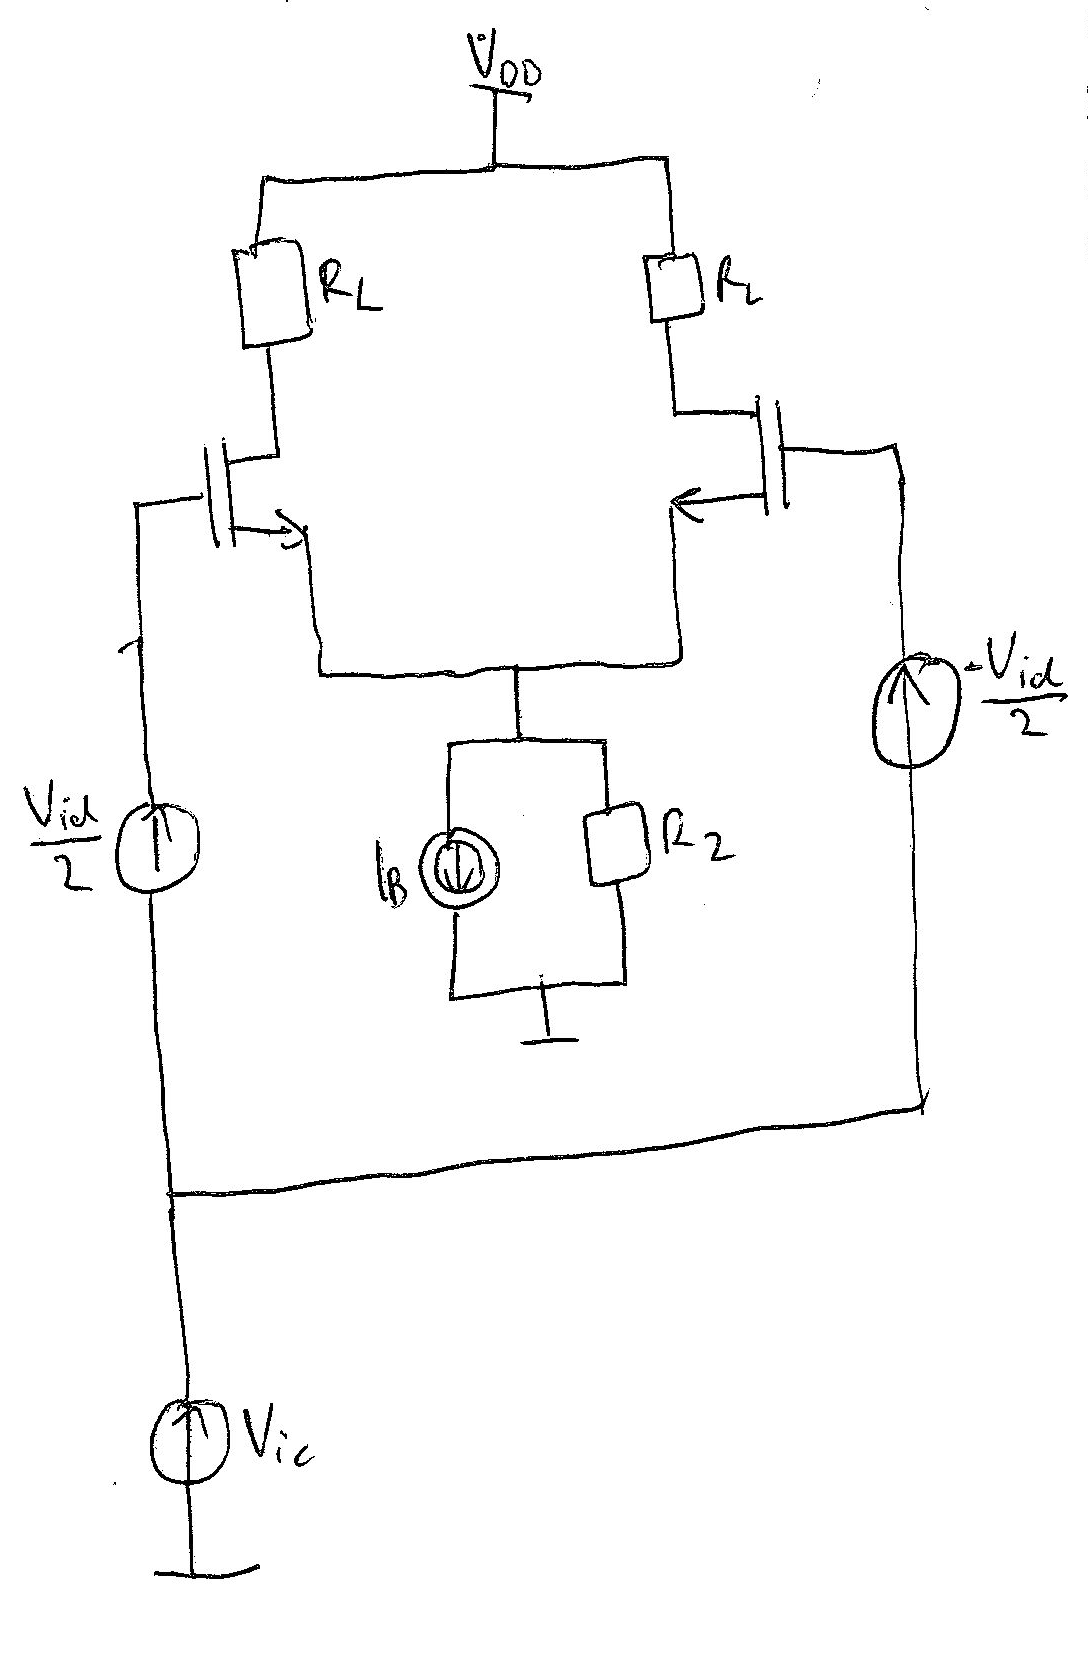
\includegraphics[width=0.35\textwidth]{roznicowy_nowe_oznaczenia.png}
\end{figure}

\subsubsection{Wzmocnienie różnicowe}

Chcemy tylko sygnał różnicowy, zwieramy więc $V_{ic}$ i zajmujemy się tylko wejściami różnicowymi.
\begin{figure}[H]
\centering
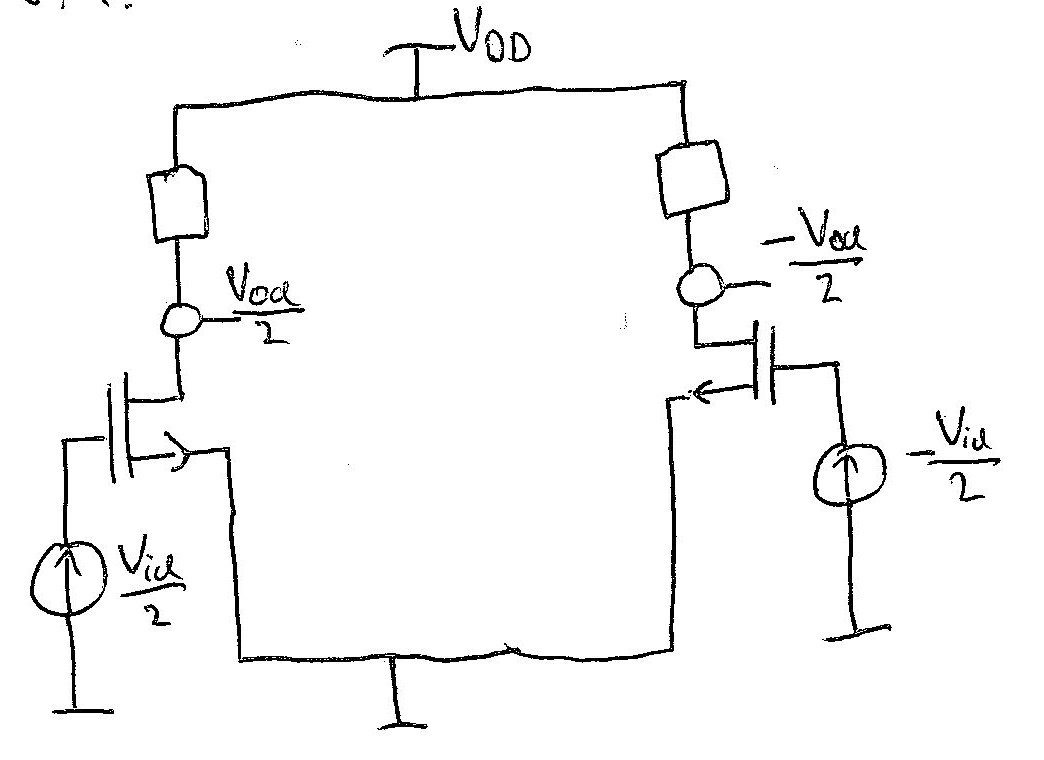
\includegraphics[width=0.5\textwidth]{roznicowy_roznica.png}
\end{figure}

Mamy tylko sygnał różnicowy. Potencjał przy gałęzi ze wspólnymi źródłami się nie zmieni przy zmianach napięcia $V_{id}$, więc zwieramy go do masy. Układ jest symetryczny, więc analizujemy tylko połówkę:
\begin{figure}[H]
\centering

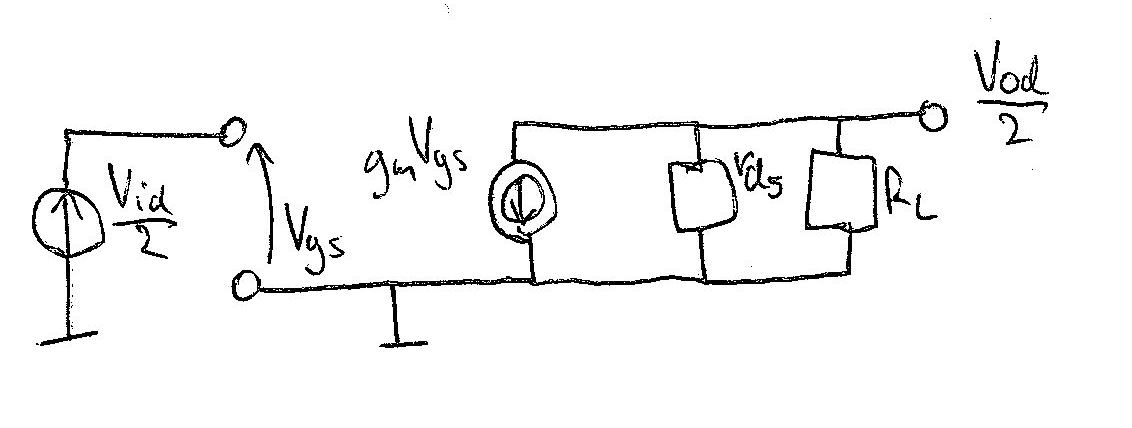
\includegraphics[width=0.5\textwidth]{roznicowy_roznica_malosyg.png}
\end{figure}

Po \textbf{prostych} obliczeniach:
\begin{align*}
\dfrac{V_{od}}{2}&=-g_{m}\dfrac{V_{id}}{2}r_{ds}\parallel R_{L} \\
A_{dm}=\dfrac{V_{od}}{V_{id}}=-g_{m} r_{ds} \parallel R_{L}
\end{align*}

$A_{dm}$ to \textbf{wzmocnienie różnicowe} (wzmocnienie układu dla symetrycznego sygnału różnicowego).

\subsubsection{Wzmocnienie sygnału współbieżnego}

Chcemy tylko sygnał współbieżny, więc tym razem zwieramy do masy oba źródła $V_{id}$. Prąd $I_{B}$ nie płynie, ponieważ mamy dwie identyczne połówki zasilane tym samym napięciem - rozwieramy. $V_{o1}$ i $V_{o2}$ są takie same. 
\begin{figure}[H]
\centering
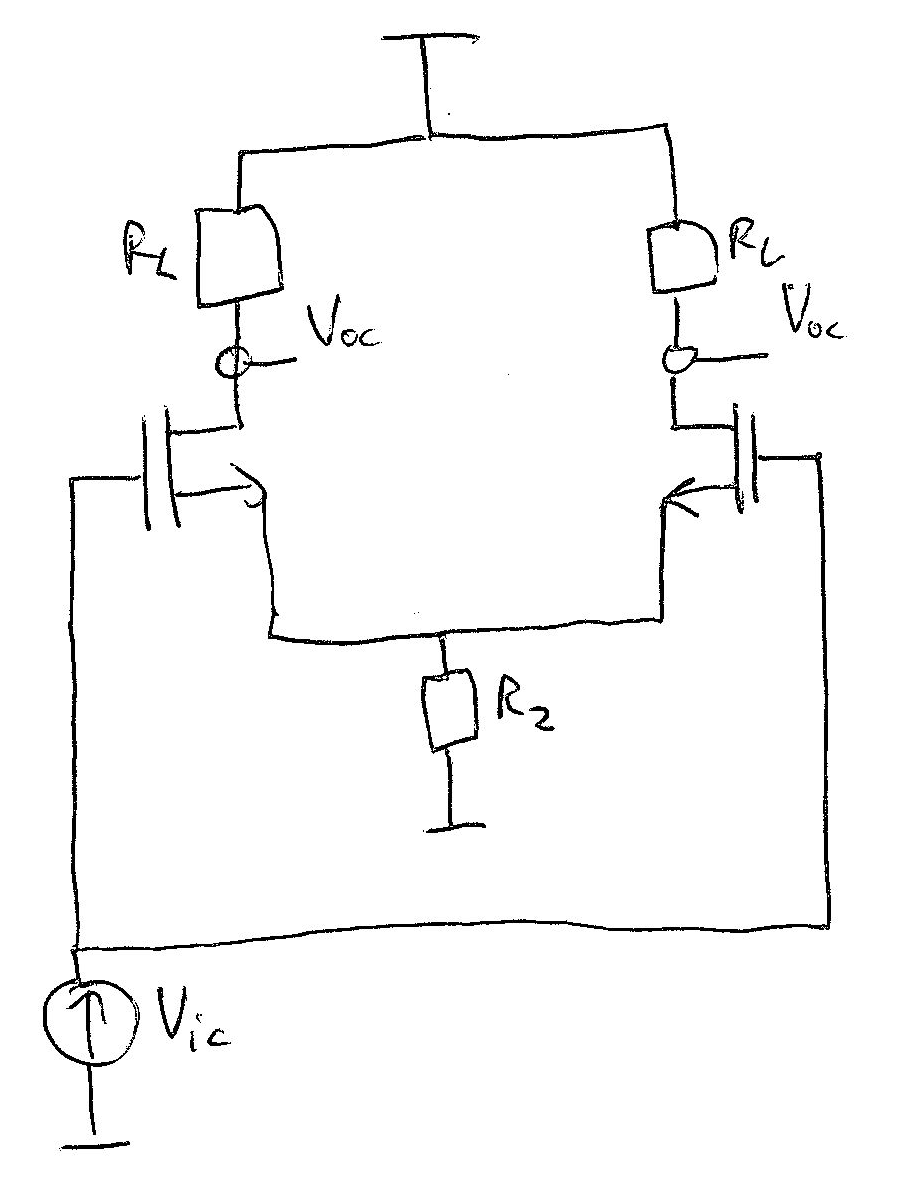
\includegraphics[width=0.35\textwidth]{roznicowy_wsp.png}
\end{figure}

Opór $R_{Z}$ musimy podzielić tak, żeby układ był symetryczny. Zastępujemy go więc równoległym połączeniem oporów $2R_{Z}$. Mamy układ symetryczny, analizujemy tylko jedną połówkę.
\begin{figure}[H]
\centering
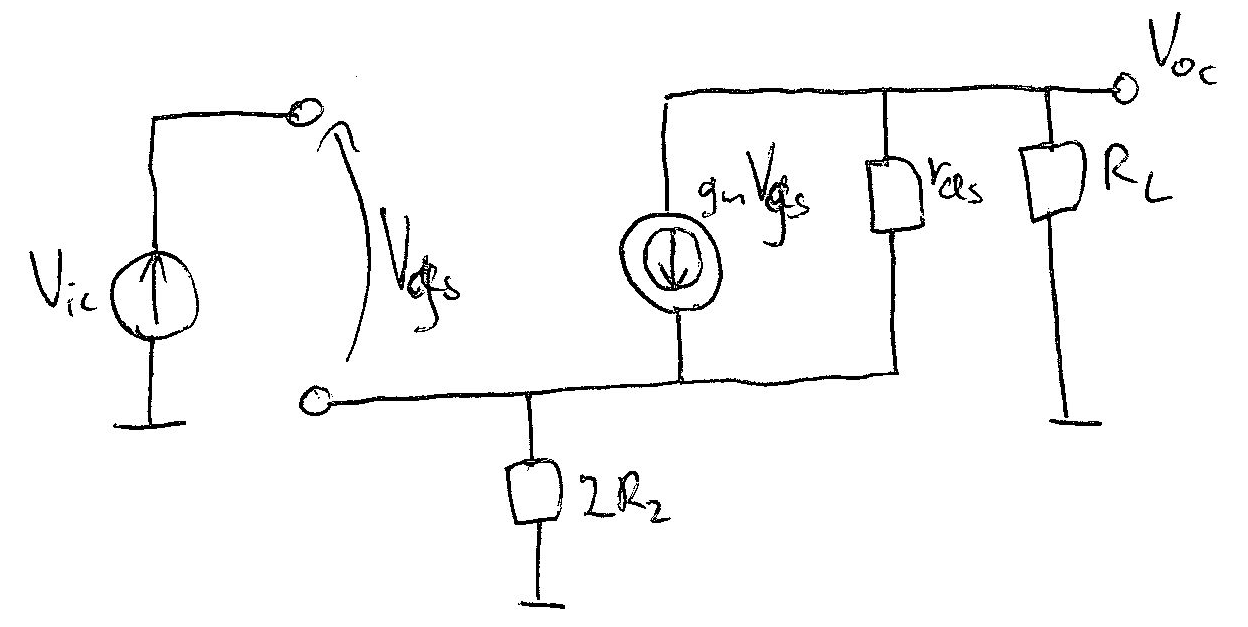
\includegraphics[width=0.5\textwidth]{roznicowy_wsp_malosyg.png}
\end{figure}

\begin{align*}
V_{oc}&=i R_L \\
[2R_{Z}+r_{ds}+R_L][i]&=[-g_{m}V_{gs}r_{ds}] \\
V_{gs}&=V_{ic}-(-i2R_{Z}) \\
[2R_{Z}+r_{ds}+R_L+2g_{m}R_{Z}r_{ds}][i]&=[-g_{m}r_{ds}V_{ic}]\\
A_{cm}=\dfrac{V_{oc}}{V_{ic}}&=\dfrac{-g_{m}R_L}{2g_{m}R_{Z}}+\dfrac{2R_{Z}+R_{L}}{r_{ds}}+1
\end{align*}

$A_{cm}$ to wzmocnienie dla sygnału współbieżnego.

\subsubsection{CMMR - współczynnik tłumienia sygnału współbieżnego}
Lepiej określa charakterystykę wzmacniacza:
\begin{equation}
CMMR=\dfrac{A_{dm}}{A_{cm}}
\end{equation}

\section{Bramki CMOS}
\subsection{Inwerter}
\begin{figure}[H]
\centering
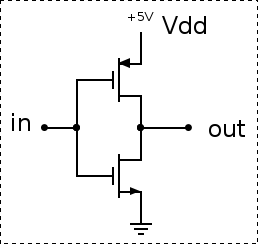
\includegraphics[width=0.35\textwidth]{NOT.png}
\end{figure}

\subsection{NAND}
\begin{figure}[H]
\centering
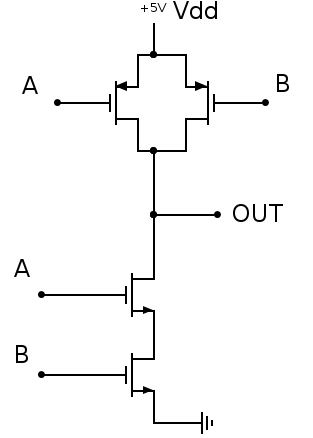
\includegraphics[height=0.35\textwidth]{NAND.png}
\end{figure}

\subsection{NOR}
\begin{figure}[H]
\centering
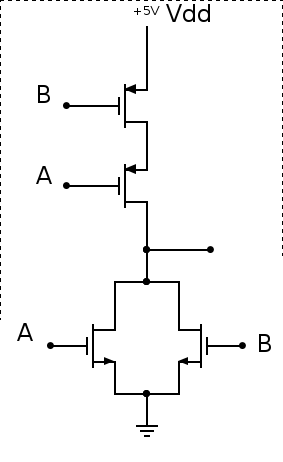
\includegraphics[height=0.35\textwidth]{NOR.png}
\end{figure}

\section{Realizacja funkcji i wymiarowanie w CMOS}
Suma (alternatywa):
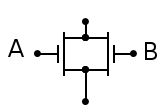
\includegraphics[width=0.25\textwidth]{suma.png}

Iloczyn (koniunkcja):
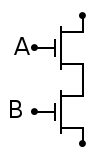
\includegraphics[width=0.25\textwidth]{iloczyn.png}

Analogicznie na pMOS-ach, z tym, że elementy są negowane.
\subsection{Jak robimy funkcję}
Najpierw musimy zbudować układ na nMOS-ach, następnie dokładnie odwrotny schemat na pMOS-ach. Najlepiej to zrozumieć na przykładzie:
Mamy funkcję np $F=A\overline{B}+C(B+D)$. Po kolei robimy poszczególne elementy korzystając z sumy i iloczynu powyżej. Budujemy układ na nMOS-ach, więc \textbf{nie możemy} dać pMOS-a jako $\overline{B}$, bo mogą się pojawić na wyjściu jakieś cząstkowe napięcia, które będą dawać fałszywą wartość logiczną. Dajemy więc nMOS-a i do niego podpinamy inwerter. 

Mamy układ na nMOS-ach, teraz musimy zrobić na pMOS-ach. Na pMOS-ach realizujemy funkcję odwrotną do zadanej - zamieniamy sumę na iloczyn, iloczyn na sumę, negujemy każdą składową, czyli $F=(\overline{A}+B)(\overline{C}+\overline{B}\overline{D})$. Negację załatwia nam tranzystor pMOS. Dla $B$ (niezanegowane), tak samo jak poprzednio, musimy wstawić inwerter. Po tym wszystkim łączymy oba układy tak, że nMOS jest na dole, pMOS na górze, w miejscu połączenia mamy funkcję $\overline{F}$ (\textbf{zanegowane!}). Do wyjścia podpinamy inwerter i mamy $F$.

\begin{figure}[H]
\centering
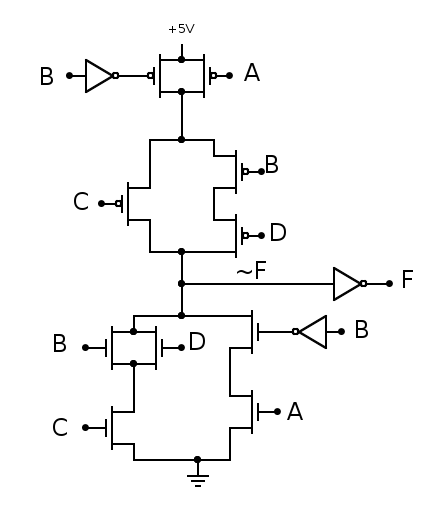
\includegraphics[height=0.5\textwidth]{F.png}
\end{figure}

\section{Wymiarowanie}
Połączenie szeregowe - mnożymy x2, równoległe - przechodzi bez zmian:
\begin{figure}[H]
\centering
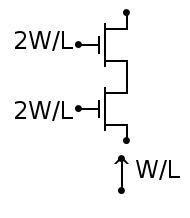
\includegraphics[width=0.35\textwidth]{wymiar_szer.png}\\
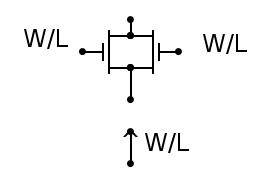
\includegraphics[width=0.35\textwidth]{wymiar_rown.png}
\end{figure}

Od dołu, na wejściu nMOS mamy $\dfrac{W}{L}$, natomiast na wejściu pMOS $\dfrac{2W}{L}$, ponieważ chcemy, żeby narastanie i opadanie było tak samo szybkie (na pMOS-ie musi być szerszy kanał).

Dla przykładu wymiarowanie powyższego układu:
\begin{figure}[H]
\centering
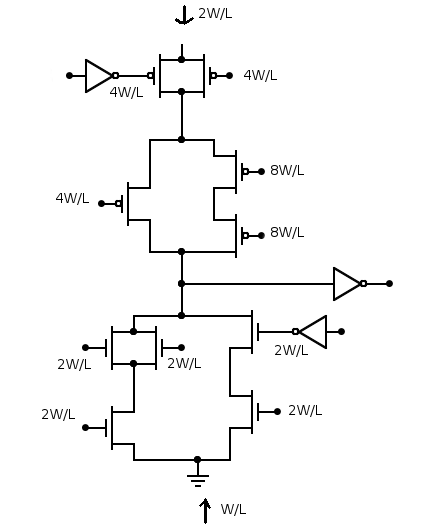
\includegraphics[width=0.5\textwidth]{F_wymiar.png}
\end{figure}

\end{document}